\documentclass[10pt,a4paper]{book}
\usepackage[utf8]{inputenc}
\usepackage[spanish]{babel}
\usepackage{graphicx}
\usepackage{amsmath}
\usepackage{amsfonts}
\usepackage{amssymb}
\usepackage{multicol}
\usepackage{multirow}
\usepackage[hidelinks]{hyperref}
\usepackage[usenames, dvipsnames]{color}
\usepackage[left=2cm,right=2cm,top=2cm,bottom=2cm]{geometry}
\title{{\Huge Modelos Lineales}}
\author{Prof. Dr. Francisco de Asís Torres Ruiz\\
		Prof. Dr. Juan José Serrano Pérez}
\date{}
\begin{document}
\maketitle
\tableofcontents

\chapter{Introducción a los Modelos Lineales y a los Modelos de Regresión}
	\section{Definición del Modelo Lineal}
Sea $Y$ una variable de la cual se desea estudiar algunos aspectos sobre su comportamiento (predecir valores futuros, comprobar si se comporta de igual manera ante influencias externas diferentes,...)

Para ese análisis consideremos un conjunto de variables \textit{auxiliares}($X_1,...,X_k$)que se cree pueden aportar información acerca del problema concreto que se desea estudiar.

Dada la naturaleza de ambos tipos de variables es usual denominar variable \emph{explicada} o \emph{dependiente} a la variable objeto de estudio, $Y$, mientras que a las otras variables se les conoce como variables \emph{explicativas} o \emph{independientes}.

Los modelos lineales adoptan tal denominación debido a que el modelo para estudiar el comportamiento de la variable dependiente vía las independientes es de la forma $$Y = \beta_0 + \beta_1X_1 + \beta_2X_2 +...+ \beta_kX_k + \epsilon$$

Para realizar el análisis que pretendemos será necesario disponer de una muestra formada por $N$, ($N > k + 1$), observaciones de dichas variables($y_i;x_{i1},...,x_{ik}$), $i=1,...,N$, las cuales verificarán las expresiones $$y_i = \beta_0 + \beta_1x_{i1} + \beta_2x_{i2} +...+ \beta_kx_{ik} + \epsilon_i\ ;\ i=1,...,N$$ que matricialmente se pueden expresar en la forma $$ \left( \begin{array}{c}
y_1\\
y_2\\
\vdots\\
y_N \end{array} \right) = 
\left( \begin{array}{cccccc}
1 & x_{11} & x_{12} & \cdots & \cdots & x_{1k} \\
1 & x_{11} & x_{12} & \cdots & \cdots & x_{1k} \\
\vdots & \vdots & \vdots & \vdots & \ddots & \vdots \\
1 & x_{N1} & x_{N2} & \cdots & \cdots & x_{Nk} \\
\end{array} \right) 
\left( \begin{array}{c}
\beta_0\\
\beta_1\\
\vdots\\
\beta_k \end{array} \right) + 
\left( \begin{array}{c}
\epsilon_1\\
\epsilon_2\\
\vdots\\
\epsilon_N \end{array} \right)$$ y en la fórmula reducida $y = X\beta + \epsilon$, donde $X$ es la llamada \textit{Matriz de Diseño}, cuyas columnas contienen las observaciones de las variables independientes más una columna de unos(si incluimos término independiente). A esta expresión genérica se le conoce como \emph{Modelo Lineal General}.

$$y_i = \beta_0 + \beta_1x_{i1} + \beta_2x_{i2} +...+ \beta_kx_{ik} + \epsilon_i\ ;\ i=1,...,N$$

En este planteamiento general quedan multitud de cuestiones por precisar como pueden ser las siguientes:
\begin{itemize}
\item La distribución de la variable de perturbación $\epsilon$
\item La aleatoriedad o no de los parámetros $\beta_j$
\item La aleatoriedad o no de las variables explicativas
\item Tipo de matriz de diseño así como su rango
\end{itemize}

Así se puede hacer una clasificación de los modelos lineales atendiendo a la naturaleza y las interrelaciones de los elementos del modelo. También se pueden clasificar según la dimensión de las variables, distinguiéndose así entre el Modelo Lineal General Univariante y Multivariante. Por último, se dirá que el modelo es
simple si sólo considera una variable explicativa, mientras que diremos que es múltiple si existen varias.

	\section{Algunos Tipos de Modelos Lineales}
$$y_i = \beta_0 + \beta_1x_{i1} + \beta_2x_{i2} +...+ \beta_kx_{ik} + \epsilon_i\ ;\ i=1,...,N$$
$$y = X\beta + \epsilon$$

\begin{itemize}
\item Se prefijan valores observados $x_1,...,x_k$ para $X_1,...X_k$
\item $Y$ observada fijados valores $x_1,...,x_k$ de las variables independientes
\item $\beta_i$ no aleatorios
\item $\epsilon_i$ aleatorios
\end{itemize}
\begin{center}
MODELOS DE REGRESIÓN CONDICIONADA\\
\textit{Modelo de Regresión Lineal}
\end{center}
\ \\
\begin{itemize}
\item $X_1,...X_k$ con valores $0$ ó $1$ que determinan condiciones del fenómeno
\item $Y$ observada para valores de las condiciones anteriores
\item $\beta_i$ no aleatorios
\item $\epsilon_i$ aleatorios
\end{itemize}
\begin{center}
MODELOS DE RELACIÓN FUNCIONAL\\
\textit{Modelos ANOVA}
\end{center}
\ \\
\begin{itemize}
\item $X_1,...,X_k$ con valores $0$ ó $1$ y valores $x_1,...,x_k$
\item $Y$ observada para valores $x_1,...,x_k$
\item $\beta_i$ no aleatorios
\item $\epsilon_i$ aleatorios
\end{itemize}
\begin{center}
MODELOS DE LA RELACIÓN FUNCIONAL\\
\textit{Diseños experimentales tipo ANCOVA}
\end{center}
\ \\
\begin{itemize}
\item $X_1,...,X_k$ con valores $0$ ó $1$ que determinan condiciones del fenómeno
\item $Y$ observada para dichas condiciones
\item $\beta_i$ no aleatorios, independientes de los términos $\epsilon_i$
\item $\epsilon_i$ aleatorios
\end{itemize}
\begin{center}
MODELOS DE LA RELACIÓN FUNCIONAL\\
\textit{Diseños experimentales de Efectos Aleatorios (Componentes de la Varianza}
\end{center}
\newpage
$$ \left( \begin{array}{c}
y_1\\
y_2\\
\vdots\\
y_N \end{array} \right) = 
\left( \begin{array}{cccccc}
1 & x_{11} & x_{12} & \cdots & \cdots & x_{1k} \\
1 & x_{11} & x_{12} & \cdots & \cdots & x_{1k} \\
\vdots & \vdots & \vdots & \vdots & \ddots & \vdots \\
1 & x_{N1} & x_{N2} & \cdots & \cdots & x_{Nk} \\
\end{array} \right) 
\left( \begin{array}{c}
\beta_0\\
\beta_1\\
\vdots\\
\beta_k \end{array} \right) + 
\left( \begin{array}{c}
\epsilon_1\\
\epsilon_2\\
\vdots\\
\epsilon_N \end{array} \right),(N > k + 1)$$
\begin{center}
$ \downarrow $
\end{center}
$$y = X\beta + \epsilon$$
\begin{center}
$ \downarrow $
\end{center}
\begin{center}
MODELO LINEAL DE GAUSS MARKOV
\end{center}

\begin{itemize}
\item $\epsilon_i$ aleatorias con media cero, varianza $\sigma^2$ e incorreladas
\item $\beta_i$ no aleatorios
\item Los valores de $X$ están prefijados
\end{itemize}

	\section{Modelo Lineal de Gauss-Markov}
$$ \left( \begin{array}{c}
y_1\\
y_2\\
\vdots\\
y_N \end{array} \right) = 
\left( \begin{array}{cccccc}
1 & x_{11} & x_{12} & \cdots & \cdots & x_{1k} \\
1 & x_{11} & x_{12} & \cdots & \cdots & x_{1k} \\
\vdots & \vdots & \vdots & \vdots & \ddots & \vdots \\
1 & x_{N1} & x_{N2} & \cdots & \cdots & x_{Nk} \\
\end{array} \right) 
\left( \begin{array}{c}
\beta_0\\
\beta_1\\
\vdots\\
\beta_k \end{array} \right) + 
\left( \begin{array}{c}
\epsilon_1\\
\epsilon_2\\
\vdots\\
\epsilon_N \end{array} \right),(N > k + 1)$$
\begin{center}
$ \downarrow $
\end{center}
$$y = X\beta + \epsilon$$
\begin{center}
$ \downarrow $
\end{center}
\begin{center}
MODELO LINEAL DE GAUSS MARKOV
\end{center}

\begin{itemize}
\item $E[\epsilon]=0,\mathrm{Cov}[\epsilon]=\sigma^2\mathbf{I}_N$
\item $\beta$ no aleatorio
\item $X$ no aleatoria
\begin{itemize}
\item $Rag(X)=k+1$. Modelo de rango completo
\item $Rag(X)<k+1$. Modelo de rango no completo
\end{itemize}
\end{itemize}
\ \\
\begin{center}
INFERENCIA
\end{center}
\begin{itemize}
\item Estimación:
\begin{itemize}
\item Mínimos cuadrados
\item Máxima verosimilitud(supuesta normalidad en los errores)
\end{itemize}
\item Contraste
\end{itemize}
\begin{center}
GENERALIZACIÓN
\ \\
Modelo de Aitken: $Cov(\varepsilon)=\sigma^2V,\ V\ conocida$
\end{center}

	\section{Ejemplos de Modelos de Gauss-Markov}
\begin{center}
PROBLEMA DE UNA MUESTRA
\end{center}
$$y \rightarrow N_1[\mu;\sigma^2] \Rightarrow y=\mu + \epsilon\  (\epsilon \rightarrow N_1[0;\sigma^2])$$
\begin{center}
$ \downarrow $
\end{center}
$$\{y_1,...,y_N\}\ m.a.s.$$
\begin{center}
$ \downarrow $
\end{center}
$$y_i=\mu + \epsilon_i\  (\epsilon_i \rightarrow N_1[0;\sigma^2])$$
\begin{center}
$ \downarrow $
\end{center}
$$ \left( \begin{array}{c}
y_1\\
\vdots\\
y_N \end{array} \right) =  
\left( \begin{array}{c}
1\\
\vdots\\
1 \end{array} \right)\mu + 
\left( \begin{array}{c}
\epsilon_1\\
\vdots\\
\epsilon_N \end{array} \right)$$
\begin{center}
$ \downarrow $
\end{center}
$$y=X\mu+\epsilon$$
\ \\
\begin{center}
PROBLEMA DE DOS MUESTRAS(rango completo)
\end{center}
\begin{center}
$y_1 \rightarrow N_1[\mu_1;\sigma^2];\ y_2 \rightarrow N_1[\mu_2;\sigma^2]$, independientes
\end{center}
\begin{center}
$ \downarrow $
\end{center}
$$\{y_{11},...,y_{1N_1}\},\ \{y_{21},...,y_{2N_2}\}\ m.a.s.$$
\begin{center}
$ \downarrow $
\end{center}
$$y_{ij}=\mu_i + \epsilon_{ij}\  (\epsilon_{ij} \rightarrow N_1[0;\sigma^2])$$
\begin{center}
$ \downarrow $
\end{center}
$$ \left( \begin{array}{c}
y_{11}\\
\vdots\\
y_{1N_1}\\
\hline
y_{21}\\
\vdots\\
y_{2N_2}\\
\end{array} \right) =  
\left( \begin{array}{cc}
1 & 0\\
\vdots & \vdots\\
1 & 0\\
\hline
0 & 1\\
\vdots & \vdots\\
0 & 1\\
\end{array} \right)
\left( \begin{array}{c}
\mu_1\\
\vdots\\
\mu_2 \end{array} \right) + 
\left( \begin{array}{c}
\epsilon_{11}\\
\vdots\\
\epsilon_{1N_1}\\
\hline
\epsilon_{21}\\
\vdots\\
\epsilon_{2N_2}\\
\end{array} \right)$$
\begin{center}
$ \downarrow $
\end{center}
$$y=X\beta+\epsilon$$
\ \\
\begin{center}
PROBLEMA DE DOS MUESTRAS(rango no completo)
\end{center}
\begin{center}
$y_1 \rightarrow N_1[\mu_1;\sigma^2];\ y_2 \rightarrow N_1[\mu_2;\sigma^2]$, independientes
\end{center}
\begin{center}
$ \downarrow $
\end{center}
$$\{y_{11},...,y_{1N_1}\},\ \{y_{21},...,y_{2N_2}\}\ m.a.s.$$
\begin{center}
$ \downarrow $
\end{center}
$$y_{ij}=\mu_i + \alpha_i + \epsilon_{ij}\  (\epsilon_{ij} \rightarrow N_1[0;\sigma^2])$$
\begin{center}
$ \downarrow $
\end{center}
$$ \left( \begin{array}{c}
y_{11}\\
\vdots\\
y_{1N_1}\\
\hline
y_{21}\\
\vdots\\
y_{2N_2}\\
\end{array} \right) =  
\left( \begin{array}{ccc}
1 & 1 & 0\\
\vdots & \vdots & \vdots\\
1 & 1 & 0\\
\hline
1 & 0 & 1\\
\vdots & \vdots & \vdots\\
1 & 0 & 1\\
\end{array} \right)
\left( \begin{array}{c}
\mu\\
\alpha_1\\
\alpha_2 \end{array} \right) + 
\left( \begin{array}{c}
\epsilon_{11}\\
\vdots\\
\epsilon_{1N_1}\\
\hline
\epsilon_{21}\\
\vdots\\
\epsilon_{2N_2}\\
\end{array} \right)$$
\begin{center}
$ \downarrow $
\end{center}
$$y=X\beta+\epsilon$$
\ \\
\begin{center}
PROBLEMA DE K MUESTRAS O ANOVA DE UNA VÍA(rango completo)
\end{center}
\begin{center}
$y_1 \rightarrow N_1[\mu_1;\sigma^2];\cdots;\ y_i \rightarrow N_1[\mu_i;\sigma^2]$, independientes
\end{center}
\begin{center}
$ \downarrow $
\end{center}
$$\{y_{11},...,y_{1N_1}\},\cdots,\{y_{i1},...,y_{iN_i};\cdots;\{y_{k1},...,y_{kN_k}\}\}\ m.a.s.$$
\begin{center}
$ \downarrow $
\end{center}
$$y_{ij}=\mu_i + \epsilon_{ij}\  (\epsilon_{ij} \rightarrow N_1[0;\sigma^2])$$
\begin{center}
$ \downarrow $
\end{center}
$$ \left( \begin{array}{c}
y_{11}\\
\vdots\\
y_{1N_1}\\
\hline
y_{21}\\
\vdots\\
y_{2N_2}\\
\hline
y_{k1}\\
\vdots\\
y_{kN_k}\\
\end{array} \right) =  
\left( \begin{array}{cccc}
1 & 0 & \cdots & 0\\
\vdots & \vdots & \vdots & \vdots\\
1 & 0 & \cdots & 0\\
\hline
\vdots & \vdots & \vdots & \vdots\\
\hline
0 & 0 & \cdots & 1\\
\vdots & \vdots & \vdots & \vdots\\
0 & 0 & \cdots & 1\\
\end{array} \right)
\left( \begin{array}{c}
\mu_1\\
\mu_2\\
\vdots\\
\alpha_k \end{array} \right) + 
\left( \begin{array}{c}
\epsilon_{11}\\
\vdots\\
\epsilon_{1N_1}\\
\hline
\epsilon_{21}\\
\vdots\\
\epsilon_{2N_2}\\
\hline
\epsilon_{k1}\\
\vdots\\
\epsilon_{kN_k}\\
\end{array} \right)$$
\begin{center}
$ \downarrow $
\end{center}
$$y=X\beta+\epsilon$$
\ \\
\begin{center}
PROBLEMA DE K MUESTRAS O ANOVA DE UNA VÍA(rango no completo)
\end{center}
$$y_{ij}=\mu + \alpha_i + \epsilon_{ij}\ (\epsilon_{ij} \rightarrow N_1[0;\sigma^2])$$
\begin{center}
$ \downarrow $
\end{center}
$$ \left( \begin{array}{c}
y_{11}\\
\vdots\\
y_{1N_1}\\
\hline
y_{21}\\
\vdots\\
y_{2N_2}\\
\hline
y_{k1}\\
\vdots\\
y_{kN_k}\\
\end{array} \right) =  
\left( \begin{array}{ccccc}
1 & 1 & 0 & \cdots & 0\\
\vdots & \vdots & \vdots & \vdots & \vdots\\
1 & 1 & 0 & \cdots & 0\\
\hline
\vdots & \vdots & \vdots & \vdots & \vdots\\
\hline
1 & 0 & 0 & \cdots & 1\\
\vdots & \vdots & \vdots & \vdots & \vdots\\
1 & 0 & 0 & \cdots & 1\\
\end{array} \right)
\left( \begin{array}{c}
\mu\\
\alpha_1\\
\alpha_2\\
\vdots\\
\alpha_k \end{array} \right) + 
\left( \begin{array}{c}
\epsilon_{11}\\
\vdots\\
\epsilon_{1N_1}\\
\hline
\epsilon_{21}\\
\vdots\\
\epsilon_{2N_2}\\
\hline
\epsilon_{k1}\\
\vdots\\
\epsilon_{kN_k}\\
\end{array} \right)$$
\begin{center}
$ \downarrow $
\end{center}
$$y=X\beta+\epsilon$$
	\section{Regresión}
\textbf{Regresión:} Búsqueda de una función que exprese la relación dos o más variables.
\ \\

\textbf{Variables:} Dependiente o explicada($Y$). Explicativas, independientes o regresores($X_1,...,X_k$)
\ \\

\textbf{Orígenes:}
\begin{itemize}
\item \textbf{Astronomía y Física:} Laplace y Gauss
\item \textbf{Biología:} Galton(acuñó el término regresión)
\end{itemize}
\textbf{Formulación del modelo:}
\begin{itemize}
\item Encontrar $g$ tal que $Y = g(X_1,...,X_k;\epsilon$)
\item \textbf{¿Quién es $g$?} Distintos tipos de regresión
\begin{itemize}
\item \textbf{Regresión lineal:} $Y = \beta_0 + \beta_1X_1 + ... + \beta_kX_k + \epsilon$
\end{itemize}
\end{itemize}

\chapter{El Modelo de Regresión Lineal Simple Univariante (I)}
	\section{Hipótesis Básicas del Modelo}
Sea $Y$ una variable que representa una característica de una población, característica objeto de estudio y sobre la cual se desea conocer diversos aspectos de su comportamiento. Para ello disponemos de la información suministrada por otra variable $X$, cuyos valores pueden ser determinados \textit{a priori}. A $Y$ la conoceremos como la variables dependiente (o variable explicada o regresando), mientras que $X$ es la
variable independiente (o variable explicativa o regresor).

Admitiremos que la hipótesis estructural básica del modelo es \textcolor{blue}{$$Y = \beta_0 + \beta_1X + \epsilon$$} o sea, la relación entre ambas variables es de tipo lineal en los parámetros del modelo. En este modelo supondremos:

\begin{itemize}
\item \textcolor{blue}{$X$ es una variable cuyos valores son conocidos al observar los valores de $Y$}
\item \textcolor{blue}{$\epsilon$ es una variable aleatoria} que engloba un conjunto de factores, cada uno de los cuales influye en la respuesta sólo en pequeña magnitud pero que de forma conjunta debe tenerse en cuenta en la especificación y tratamiento del modelo.
\item \textcolor{blue}{$\beta_0$ y $\beta_1$ son constantes fijas(no aleatorias)} pero desconocidas, cuyos valores deberán ser estimados.
\end{itemize}

Como hemos dicho anteriormente, para cada valor xi fijo de la variable independiente (condición experimental) se dispondrá de una realización de la variable dependiente. Por lo tanto tendremos una muestra de pares de valores ($x_i,y_i$), $i=1,...,N$ ($N > 2$).

Dada la estructura funcional impuesta del modelo, para cada valor $x_i$ fijo se verifica $$y_i=\beta_0 + \beta_1x_i + \epsilon_i\ ;\ i=1,...,N$$ donde las variables $\epsilon_i$ (perturbaciones) se consideran realizaciones de la variable de error $\epsilon$.

Notemos que en lo que hasta ahora se ha dicho ya hay una serie de hipótesis establecidas. Además de ellas, se añaden las siguientes hipótesis sobre las variables de perturbación y la variable explicativa o independiente:
\begin{itemize}
\item Las perturbaciones tienen media cero \textcolor{blue}{$$E[\epsilon_i]=0\ ;\ i=1,...,N$$}
\item Las perturbaciones tienen varianza constante(hipótesis de homocedasticidad)\textcolor{blue}{$$\mathrm{Var}[\epsilon_i]=\sigma^2\ ;\ i=1,...,N$$}
\item Las perturbaciones son incorreladas entre sí(hipótesis de incorrelación) \textcolor{blue}{$$\mathrm{Cov}[\epsilon_i,\epsilon_j]=E[\epsilon_i\epsilon_j]=0\ ;\ i,j=1,...,N\ (i\neq j)$$}
\item Los valores de la variable $X$ no son todos iguales, o sea, al menos hay dos observaciones distintas o, lo que es lo mismo, la variable \textcolor{blue}{$X$ es no degenerada}.
\end{itemize}

\textbf{Nota 1.1.} \textit{Observemos que la formulación del modelo, junto con las hipótesis establecidas nos conduce a un modelo lineal de Gauss-Markov con matriz de diseño} $$X=\left( \begin{array}{cc}
1 & x_1\\
1 & x_2\\
\vdots & \vdots\\
\vdots & \vdots\\
0 & x_N\\
\end{array} \right)$$
\textit{Puesto que la variable explicativa es no degenerada, las columnas de dicha matriz no pueden ser proporcionales y con ello su rango es 2. Por lo tanto el modelo es de rango completo.}
\ \\

Las hipótesis que atañen a las variables perturbación pueden ser formuladas en términos de la variable explicada puesto que del hecho de que la variable explicativa sea no aleatoria (ni los efectos tampoco) se desprende que toda la carga aleatoria del modelo descansa sobre las variables de perturbación y por lo tanto la variable Y retoma el carácter aleatorio de ellas. Así se pueden expresar las tres primeras hipótesis anteriores en la forma siguiente:
\begin{itemize}
\item La esperanza de la respuesta depende linealmente de $X$: \textcolor{blue}{$E[y_i]=\beta_0 + \beta_1x_i\ ;\ i=1,...,N$}\\
{\scriptsize Realmente deberíamos escribir $E[y_i | X=x_i]=\beta_0 + \beta_1x_i\ ;\ i=1,...,N$}
\item La varianza de las variables $y_i$ es constante: \textcolor{blue}{$\mathrm{Var}[y_i]=\sigma^2\ ;\ i=1,...,N$}
\item Las observaciones $y_i$ son incorreladas entre sí: \textcolor{blue}{$\mathrm{Cov}[y_i,y_j]=0\ ;\ i,j=1,...,N\ (i \neq j)$}
\end{itemize}

\textbf{Nota 1.2.} \textit{$\beta_0$ representa el valor medio de la variable $Y$ cuando la variable $X$ vale cero. Asimismo $\beta_1$ es el incremento que experimenta la media de $Y$ cuando $X$ aumenta en una unidad.}

El modelo incluye otra hipótesis, si bien no es preciso para todo lo que se va a realizar sobre él. En concreto no hará falta en lo que concierne a la estimación del modelo por el método de mínimos cuadrados (si bien sí la hará cuando la estimación se realiza por máxima verosimilitud), aunque resultará imprescindible en el momento en que sean necesarias las distribuciones de los estadísticos involucrados en el proceso para establecer contrastes de hipótesis e intervalos de confianza. Esta hipótesis es la siguiente:
\begin{itemize}
\item \textcolor{blue}{Las variables de perturbación son independientes y están igualmente distribuidas según una ley normal de media 0 y varianza $\sigma^2$}
\end{itemize}

Asimismo se puede reformular esta hipótesis refiriéndola a las variables $y_i$:
\begin{itemize}
\item \textcolor{blue}{La distribución de $y_i$, para cada $x_i$, es normal de media $\beta_0 + \beta_1x_i$ y varianza $\sigma^2$, siendo todas las distribuciones independientes}
\end{itemize}

\subsection{Comentarios a las Hipótesis del Modelo}
\begin{enumerate}
\item La hipótesis principal del modelo es que la media de la distribución de $Y$, para cada valor de $X$ fijo, varía de forma lineal con dicho valor. Esta hipótesis, en la medida que se pueda, debe ser comprobada siempre ya que condiciona toda la construcción del modelo. En cualquier caso conviene tener en cuenta que una relación lineal debe considerarse en general como una aproximación simple, en un rango limitado, a una relación más compleja. En consecuencia, es necesario tener presente el rango de valores dentro del cual se va a trabajar y el peligro de extrapolar la relación fuera de ese rango.
\item La hipótesis de homocedasticidad no se cumplirá si la variabilidad depende, por ejemplo, de las observaciones de la variable independiente. Por ejemplo, si se pretende estudiar el ahorro en función de la renta en varias familias, podemos fácilmente pensar que la variabilidad del ahorro dependerá, de forma fuerte, del nivel de renta de las familias ya que, a renta superior, una familia tiene una mayor flexibilidad a la hora de qué hacer con su dinero, teniendo la posibilidad de ahorrar o consumir, mientras que las familias de renta inferior tendrán menos posibilidades de ahorrar, moviéndose por lo tanto en una franja más estrecha y menos flexible.
\item La incorrelación entre las perturbaciones es esperable en situaciones estáticas, o sea, cuando las observaciones
correspondan al mismo periodo temporal, pero no lo será tanto en situaciones dinámicas
en las que se mide la variable respuesta a lo largo del tiempo. Por ejemplo, si pretendemos estudiar dos variables de índole económica en distintos países durante un mismo año, como pueden ser el producto interior bruto como variable independiente y el consumo como variable dependiente, es de suponer, en principio, que no tiene por qué haber una dependencia entre las observaciones. Sin embargo ese mismo tipo de estudio hecho en un país concreto a lo largo de varios años puede llevar implícito el hecho de que los factores recogidos en la perturbación hayan evolucionado en el tiempo y, por lo tanto, haya algún tipo de correlación a lo largo del tiempo entre las perturbaciones.
\end{enumerate}
	\section{Estimación del Modelo por Mínimos Cuadrados Ordinarios}
		\subsection{Obtención de Estimadores}
Consideremos el modelo de regresión lineal simple $Y=\beta_0 + \beta_1X + \epsilon$

Nuestra intención es encontrar los valores de $\beta_0$ y $\beta_1$ tales que expliquen de la mejor forma posible la relación de tipo lineal que liga a las variables en estudio. Para ello tendremos que buscar dos estimaciones de dichos parámetros, llamémoslas $\widehat{\beta_0}$ y $\widehat{\beta_1}$

Bajo este supuesto, y para cada valor de $x$ de $X$, la predicción que sobre la variable $Y$ se haría es $$\widehat{y}=\widehat{\beta_0}+\widehat{\beta_1}x$$ expresión que genera, al variar $X$ en su rango, una recta, llamada \textit{recta de regresión}.

Para realizar el proceso de estimación necesitamos una muestra de la variable dependiente. Cada elemento de dicha muestra se obtiene fijado un valor $x_i$ de $X$. De esta forma tenemos las relaciones $$y_i=\beta_0+\beta_1x_i+\epsilon_i\ ;\ i=1,...,N,\ (N > 2)$$

A continuación debemos fijar un criterio para la estimación. En primer lugar emplearemos el criterio de mínimos cuadrados ordinarios, según el cual hemos de minimizar, en $\beta_0$ y $\beta_1$, la suma de los cuadrados de los errores. Es decir, el problema que hay que resolver es  $$\operatorname*{Min}\limits_{\beta_0,\beta_1}\sum^N_{i=1}\epsilon^2_i$$ 

Intuitivamente podemos observar que lo que se hace es minimizar el efecto de las perturbaciones de forma global(piénsese en el hipotético caso en que esa suma valiera cero).

Matemáticamente hablando el problema se traduce en minimizar la función de dos variables $$ S(\beta_0,\beta_1)=\sum_{i=1}^N\epsilon_i^2=\sum_{i=1}^N(y_i-\beta_0-\beta_1x_i)^2$$

Para la resolución técnica se deriva la función anterior respecto de los parámetros y se plantea el sistema de ecuaciones  $$\frac{\partial S(\beta_0,\beta_1)}{\partial \beta_0}=0, \qquad \frac{\partial S(\beta_0,\beta_1)}{\partial \beta_1}=0$$ resultando así $$-2\sum^N_{i=1}(y_i\beta_0-\beta_1x_i)=0,\qquad -2\sum^N_{i=1}(y_i-\beta_0-\beta_1x_i)x_i=0$$ o lo que es lo mismo $$\sum^N_{i=1}\epsilon_i=0,\qquad \sum^N_{i=1}\epsilon_ix_i=0$$ que da origen al denominado sistema de ecuaciones normales $$\sum^N_{i=1}y_i=N\beta_0+\beta_1\sum^N_{i=1}x_i$$ $$\sum^N_{i=1}y_ix_i=\beta_0\sum^N_{i=1}x_i+\beta_1\sum^N_{i=1}x_i^2$$

Llamando $\widehat{\beta_0}$ y $\widehat{\beta_1}$ a la solución del sistema, esta es: $$\widehat{\beta_1}=\frac{s_{xy}}{s^2_x}$$ $$\widehat{\beta}_0=\bar{y}-\frac{s_{xy}}{s^2_x}\bar{x}$$

Además, la matriz hessiana, en el punto ($\widehat{\beta}_0,\widehat{\beta}_1$), es $$H(\widehat{\beta}_0,\widehat{\beta}_1)= \left( \begin{array}{cc}
2N & 2N\bar{x}\\
 & \\
2N\bar{x} & 2\displaystyle\sum^N_{i=1}x^2_i\\
 & 
\end{array} \right)$$ matriz que claramente es definida positiva, gracias a la hipótesis establecida sobre la variable explicativa, puesto que su determinante es $4N^2s^2_x$.
\ \\

\textcolor{red}{EJERCICIO: Plantear, resolver el sistema de ecuaciones normales y comprobar que la solución minimiza la función objetivo.}
\ \\

De esta forma la recta de regresión estimada queda en la forma \textcolor{blue}{$$\widehat{y}-\bar{y}=\frac{s_{xy}}{s^2_x}(x-\bar{x})$$}

Definimos ahora los residuos mínimo-cuadráticos como la diferencia entre el valor real observado de la variable dependiente y el predicho por la recta de regresión, es decir $$e_i=y_i-\widehat{y}_i=(y_i-\bar{y})-\frac{s_{xy}}{s^2_x}(x_i-\bar{x})$$ con lo cual se puede concluir que el valor mínimo que alcanza la función $S(\beta_0,\beta_1)$ es $\displaystyle\sum^N_{i=1}e^2_i$.
De la anterior expresión para los residuos se puede deducir lo siguiente: $$\sum^N_{i=1}e_i=0,\quad \bar{\widehat{y}}=\bar{y},\qquad \sum^N_{i=1}x_ie_i=0,\qquad \sum^N_{i=1}(\widehat{y}-\bar{y})e_i=0$$
\ \\

\textcolor{red}{EJERCICIO: Verificar estas igualdades partiendo de la expresión anterior para $e_i$.} 
\ \\

De dichas relaciones se puede concluir que $y_i=\widehat{y}_i + e_i$, donde $\widehat{y}_i$ es la parte estimada y $e_i$ es la parte residual debida a la regresión, siendo ambas incorreladas.
\ \\

\textcolor{red}{EJERCICIO: Realizar la estimación m.c. en el modelo sin término constante: $Y = \beta_1X + \varepsilon$.}
		\subsection*{COMPLEMENTO: Caso de Datos Repetidos}
En muchas ocasiones la experiencia que se pretende estudiar se diseña de forma que, para cada valor fijado de la variable explicativa, se observan diversos valores de la variable dependiente. Nosotros nos referiremos a esta situación con el nombre de \textit{datos repetidos}.

Si suponemos que son $d$, $d > 2$, los valores distintos de la variable explicativa fijados y que, para cada uno, se observan $n_i$ valores de la variable dependiente, los datos suelen presentarse en la forma $$\begin{array}{c|cccc}
x_1 & y_{11} & \cdots & \cdots & y_{1n_1} \\
x_2 & y_{21} & \cdots & \cdots & y_{2n_2}  \\
\vdots & \vdots & \vdots & \vdots & \vdots \\
x_d & y_{d1} & \cdots & \cdots & y_{dn_d}  \\
\end{array}$$

Gráficamente
\begin{center}
\begin{picture}(300,180)
%Ejes X e Y
\put(0,10){\line(1,0){300}}
\put(0,10){\line(0,1){180}}

%X_i
\put(40,0){$x_1$}
\put(110,0){$x_2$}
\put(180,0){$x_i$}
\put(250,0){$x_d$}

\color{red}{
%Puntos X_1
\put(45,40){\circle*{5}}
\put(45,60){\circle*{5}}
\put(45,120){\circle*{5}}
\put(45,140){\circle*{5}}

%Puntos X_2
\put(115,50){\circle*{5}}
\put(115,60){\circle*{5}}
\put(115,120){\circle*{5}}
\put(115,140){\circle*{5}}
\put(115,160){\circle*{5}}

%Puntos X_i
\put(185,40){\circle*{5}}
\put(185,70){\circle*{5}}
\put(185,80){\circle*{5}}
\put(185,130){\circle*{5}}

%Puntos X_d
\put(255,100){\circle*{5}}
\put(255,115){\circle*{5}}
\put(255,130){\circle*{5}}
\put(255,150){\circle*{5}}
}

\color{black}{
%y_i
\put(190,38){$y_{i2}$}
\put(190,68){$y_{i3}$}
\put(190,78){$y_{in_i}$}
\put(190,128){$y_{i1}$}
}
\end{picture}
\end{center}

El modelo se escribe en la forma $y_{ij}=\beta_0+\beta_1x_i+\epsilon_{ij},\, i=1,...,d;\, j=1,...,n_i$

Notemos que no estamos tratando con un modelo distinto sino con el mismo anterior que se ha reescrito acorde con la estructura de los datos. No obstante, es interesante desarrollar de nuevo la estimación mínimo-cuadrática en esta forma para asentar mejor la idea de la regresión al comprobar qué es lo que hace el modelo en esta situación.

La función que hay que minimizar se escribe ahora como $$S(\beta_0,\beta_1)=\sum^d_{i=1}\sum^{n_i}_{j=1}(y_{ij}-\beta_0-\beta_1x_i)^2$$

Razonando igual que antes se llega al sistema de ecuaciones normales $$\sum^d_{i=1}n_i\bar{y}_i=N\beta_0+\beta_1\sum^d_{i=1}n_ix_i$$ $$\sum^d_{i=1}n_i\bar{y}_ix_i=\beta_0\sum^d_{i=1}n_ix_i+\beta_1\sum^d_{i=1}n_ix_i^2$$ cuya solución, obviamente, es la misma obtenida anteriormente.

\textbf{En este caso la estimación considera la nube de puntos} $\mathbf{\{x_i,\bar{y}_i\}_{i=1,...,d}}$ \textbf{, tratando cada punto con la frecuencia} $\mathbf{n_i}$ \textbf{observada.}
\ \\
\begin{center}
\begin{picture}(300,180)
%Ejes X e Y
\put(0,10){\line(1,0){300}}
\put(0,10){\line(0,1){180}}

%X_i
\put(40,0){$x_1$}
\put(110,0){$x_2$}
\put(180,0){$x_i$}
\put(250,0){$x_d$}

\color{red}{
%Puntos X_1
\put(45,40){\circle*{5}}
\put(45,60){\circle*{5}}
\put(45,120){\circle*{5}}
\put(45,140){\circle*{5}}

%Puntos X_2
\put(115,50){\circle*{5}}
\put(115,60){\circle*{5}}
\put(115,120){\circle*{5}}
\put(115,140){\circle*{5}}
\put(115,160){\circle*{5}}

%Puntos X_i
\put(185,40){\circle*{5}}
\put(185,70){\circle*{5}}
\put(185,80){\circle*{5}}
\put(185,130){\circle*{5}}

%Puntos X_d
\put(255,100){\circle*{5}}
\put(255,115){\circle*{5}}
\put(255,130){\circle*{5}}
\put(255,150){\circle*{5}}
}

\color{black}{
%y_i
\put(190,38){$y_{i2}$}
\put(190,68){$y_{i3}$}
\put(190,78){$y_{in_i}$}
\put(190,128){$y_{i1}$}
}

\color{blue}{
%Medias
\put(39,95){\circle*{5}}
\put(109,110){\circle*{5}}
\put(178,90){\circle*{5}}
\put(248,121){\circle*{5}}
}

\color{green}{
%Línea de ajuste
\put(0,65){\line(4,1){280}}
}

\end{picture}
\end{center}

Asimismo las relaciones obtenidas para los residuos, $e_{ij}=y_{ij}-\widehat{y_i}$, siguen siendo ciertas $$\sum^d_{i=1}\sum^{n_i}_{j=1}e_{ij}=0,\quad \bar{\widehat{y}}=\bar{y}, \quad \sum^d_{i=1}\sum^{n_i}_{j=1}e_{ij}x_{ij}=0, \quad \sum^d_{i=1}\sum^{n_i}_{j=1}(\bar{\widehat{y}}-\bar{y})e_{ij}=0$$
\ \\

\textcolor{red}{EJERCICIO: Desarrollar la estimación mínimo-cuadrática del modelo y verificar las propiedades de los residuos.}

		\subsection{Interpretación Geométrica del Método de Mínimos Cuadrados}
El método de mínimos cuadrados tratado anteriormente admite una fácil y simple interpretación geométrica. Para expresar vectorialmente el conjunto de observaciones y predicciones definamos los vectores siguientes $$y=(y_1,...,y_N)^t,\qquad \mathbf{1}=(1,...,1)^t,\qquad x=(x_1,...,x_N)^t$$ $$\varepsilon=(\epsilon_1,...,\epsilon_N)^t,\qquad e=(e_1,...,e_N)^t,\qquad \widehat{y}=(\widehat{y}_1,...,\widehat{y}_N)^t$$

Con esta notación el modelo queda en la forma $y=\beta_0\mathbf{1}+\beta_1x+\varepsilon$

Estimar los parámetros por mínimos cuadrados ordinarios requiere encontrar constantes $\widehat{\beta}_0$ y $\widehat{\beta}_1$ tales que el módulo del vector $\varepsilon$ sea mínimo. Por lo tanto se trata de determinar un vector $\widehat{y}$, en el plano definido por los vectores $\mathbf{1}$ y $x$ en un espacio$N$-dimensional, tal que el módulo del vector sea $\varepsilon$ sea mínimo.
\begin{center}
\begin{picture}(600,180)
\put(50,0){\line(1,0){300}}\put(50,0){\line(2,3){100}}\put(350,0){\line(2,3){100}}\put(365,0){$<$\textbf{1, x}$>$}
\thicklines{

\put(160,50){\vector(1,2){66}}\put(205,160){\textbf{y}}
\color{green}{
	\put(160,50){\vector(4,-1){120}}
	\put(280,20){\vector(-1,3){54}}
	\put(248,120){$\epsilon$}
	\put(242,30){\framebox(30,10){\color{black}{{\tiny $\beta_0+\beta_1\mathbf{X}$}}}}}
	
\color{red}{
	\put(160,50){\vector(1,0){150}}
	\put(310,50){\vector(-2,3){87}}
	\put(252,140){$\epsilon$}
	\put(270,52){\framebox(30,10){\color{black}{{\tiny $\beta_0+\beta_1\mathbf{X}$}}}}}
	
\color{blue}{
	\put(156,50){\vector(2,1){150}}
	\put(306,124){\vector(-3,2){85}}
	\put(254,160){$\epsilon$}
	\put(263,121){\framebox(30,10){\color{black}{{\tiny $\beta_0+\beta_1\mathbf{X}$}}}}}
	
}
\end{picture}
\end{center}

La solución es tomar la proyección ortogonal del vector $y$ sobre este plano, ya que cualquier otro caso conduciría a un vector residual de módulo mayor. Con ello el vector $\varepsilon$ será perpendicular a todos los vectores de dicho plano, bastando para ello con que lo sean con los vectores que lo generan, o sea, los vectores $\mathbf{1}$ y $x$. Así tendrá
\begin{center}
\begin{picture}(600,180)
\put(50,0){\line(1,0){300}}\put(50,0){\line(2,3){100}}\put(350,0){\line(2,3){100}}\put(365,0){$<$\textbf{1, x}$>$}
\thicklines{

\put(160,50){\vector(1,2){66}}\put(205,160){\textbf{y}}
\color{green}{
	\put(160,50){\vector(4,-1){120}}
	\put(280,20){\vector(-1,3){54}}
	\put(248,120){$\epsilon$}
	\put(242,30){\framebox(30,10){\color{black}{{\tiny $\beta_0+\beta_1\mathbf{X}$}}}}}
	
\color{red}{
	\put(160,50){\vector(1,0){150}}
	\put(310,50){\vector(-2,3){87}}
	\put(252,140){$\epsilon$}
	\put(270,52){\framebox(30,10){\color{black}{{\tiny $\beta_0+\beta_1\mathbf{X}$}}}}}
	
\color{blue}{
	\put(156,50){\vector(2,1){150}}
	\put(306,124){\vector(-3,2){85}}
	\put(254,160){$\epsilon$}
	\put(263,121){\framebox(30,10){\color{black}{{\tiny $\beta_0+\beta_1\mathbf{X}$}}}}}
	
\color{BurntOrange}{
	\put(150,50){\vector(3,2){67}}
	\put(216,95){\vector(0,1){85}}
	\put(210,140){$\epsilon$}
	\put(182,96){\framebox(30,10){\color{black}{{\tiny $\widehat{\beta}_0+\widehat{\beta}_1\mathbf{X}$}}}}}
	
}
\end{picture}
\end{center}
lo que se traduce en $$\varepsilon'\mathbf{1}=0 \Leftrightarrow \sum^N_{i=1}\epsilon_i=0$$ $$\varepsilon'x=0 \Leftrightarrow \sum^N_{i=1}\epsilon_ix_i=0$$ lo cual conduce al sistema de ecuaciones normales obtenido anteriormente.

Notemos asimismo que el triángulo resultante de la proyección indica que $\parallel y\parallel^2=\parallel e\parallel ^2+\parallel \widehat{y}\parallel ^2$ o, lo que es lo mismo, $$\sum^N_{i=1}y^2_i=\sum^N_{i=1}e_i^2+\sum^N_{i=1}\widehat{y}_i^2$$
		\subsection{Propiedades de los Estimadores Mínimo-Cuadráticos de la Recta de Regresión}
\underline{\textbf{Los estimadores son lineales}}

A partir de la expresión de $\widehat{\beta}_1$ podemos escribir: $$\widehat{\beta}_1=\dfrac{s_{xy}}{s^2_x}=\dfrac{\displaystyle\sum^N_{i=1}(x_i-\bar{x})(y_i-\bar{y})}{Ns^2_x}=\dfrac{\displaystyle\sum^N_{i=1}(x_i-\bar{x})y_i}{Ns^2_x}=\displaystyle\sum^N_{i=1}w_iy_i,\quad \mathrm{donde}\quad w_i=\dfrac{x_i-\bar{x}}{Ns^2_x}$$

Observamos por tanto que $\widehat{\beta}_1$ es un \textbf{estimador residual} en las variables $y_i$

Usando la expresión del modelo, tenemos 
\begin{center}
$\displaystyle\sum^N_{i=1}w_iy_i=\displaystyle\sum^N_{i=1}(\beta_0+\beta_1x_i+\epsilon_i)=\beta_1+\displaystyle\sum^N_{i=1}w_i\epsilon_i\qquad$ \textcolor{red}{$\displaystyle\sum^N_{i=1}w_i=0,\: \displaystyle\sum^N_{i_1}w_ix_i=1$}
\end{center}

Así pues, $\widehat{\beta}_1$ también puede expresarse como \textbf{combinación lineal} de las variables de perturbación $\epsilon_i$.

Por otro lado $$\widehat{\beta}_0=\bar{y}-\widehat{\beta}_1\bar{x}=\dfrac{1}{N}\sum^N_{i=1}y_i-\bar{x}\sum^N_{i=1}w_iy_i=\sum^N_{i=1}\left[\dfrac{1}{N}-\bar{x}w_i\right] y_i=\sum^N_{i=1}\left[\dfrac{1}{N}-\bar{x}w_i\right] (\beta_0+\beta_1x_i+\epsilon_i)=\beta_0+\sum^N_{i=1}\left[\dfrac{1}{N}-\bar{x}w_i\right]\epsilon_i$$ donde se ha usado ahora que \textcolor{red}{$\displaystyle\sum^N_{i=1}\left[\dfrac{1}{N}-\bar{x}w_i\right]=1$} y \textcolor{red}{$\displaystyle\sum^N_{i=1}\left[\dfrac{1}{N}-\bar{x}w_i\right]x_i=0$}

Por tanto, $\widehat{\beta}_0$ también es combinación lineal tanto de las variables $y_i$ como de las perturbaciones $\epsilon_i$.
\ \\

\underline{\textbf{Los estimadores son insesgados}}

De las relaciones anteriores se deduce inmediatamente la insesgadez de ambos estimadores, esto es $E[\widehat{\beta}_0]=\beta_0$ y $E[\widehat{\beta}_1]=\beta_1$
\ \\

\underline{\textbf{Varianzas y covarianza de los estimadores}}

Como $\widehat{\beta}_1$ es un estimador insesgado para $\beta_1$ se tiene $$\mathrm{Var}[\widehat{\beta}_1]=E[(\widehat{\beta}_1-\beta_1)^2]=E\left[\left(\sum^N_{i=1}w_i\epsilon_i \right) ^2\right] =E\left[\sum^N_{i=1}w^2_i\epsilon^2_i+\sum^N_{i,j=1\atop i\ne j}w_iw_j\epsilon_i\epsilon_j\right]=\sum^N_{i=1}w_i^2E[\epsilon^2_i]+\sum^N_{i,j=1\atop i\ne j}w_iw_jE[\epsilon_i\epsilon_j]=$$$$=\sigma^2\sum^N_{i=1}w^2_i=\sigma^2\sum^N_{i=1}\dfrac{(x_i-\bar{x})^2}{N^2(s^2_x)^2}=\dfrac{\sigma^2}{Ns^2_x}$$

\begin{itemize}
\item El error de estimación es inversamente proporcional a la dispersión de los valores de la variable $X$
\item El error de estimación es directamente proporcional a $\sigma^2$ o variabilidad intrínseca de la variable respuesta para cada de $X$ fijo
\end{itemize}

Razonando de forma análoga a la anterior se tiene $$\mathrm{Var}[\widehat{\beta}_0]=E[(\widehat{\beta}_0-\beta_0)^2]=E\left[\left(\sum^N_{i=1}\left[\dfrac{1}{N}-\bar{x}w_i\right]\epsilon_i\right)^2\right]=\cdots=\sigma^2\left[\dfrac{1}{N}+\dfrac{\bar{x}^2}{Ns^2_x}\right]$$

Esta expresión muestra la varianza de $\widehat{\beta}_0$ como suma de dos términos: el primero es el error de estimación de la media de la variable $Y$, mientras que el segundo tiene en cuenta que el error de la estimación de la pendiente de la recta se transmite a la ordenada en el origen (recuérdese cómo se ha obtenido este estimador) en función de lo alejado que se encuentre $\bar{x}$ del origen.
\ \\

\textcolor{red}{EJERCICIO: Realizar el desarrollo del cálculo de $\mathrm{Var}[\widehat{\beta}_0]$.}
\ \\

En cuanto a la covarianza tenemos 
\begin{equation*}\begin{split}\mathrm{Cov}[\widehat{\beta}_0,\widehat{\beta}_1]&=E[(\widehat{\beta}_0-\widehat{\beta}_0)(\widehat{\beta}_1-\widehat{\beta}_1)]=E\left[\left(\sum^N_{i=1}\left[\dfrac{1}{N}-\bar{x}w_i\right]\epsilon_i\right)\left(\sum^N_{j=1}w_j\epsilon_j\right)\right]\\&=E\left[\sum^N_{i=1}\sum^N_{j=1}\left[\dfrac{1}{N}-\bar{x}w_i\right]w_j\epsilon_i\epsilon_j\right]=\sum^N_{i=1}\sum^N_{j=1}\left[\dfrac{1}{N}-\bar{x}w_i\right]w_jE[\epsilon_i\epsilon_j]\\&=\sigma^2\sum^N_{i=1}\left[\dfrac{1}{N}-\bar{x}w_i\right]w_i=\sigma^2\sum^N_{i=1}\left[\dfrac{x_i-\bar{x}}{N^2s^2_x}-\bar{x}\dfrac{(x_i-\bar{x})^2}{N^2(s^2_x)^2}\right]=-\sigma^2\dfrac{\bar{x}}{Ns^2_x}\end{split} 
\end{equation*}

Con ello se observa que si $\bar{x}$ es mayor que cero entonces errores por exceso en la estimación de la pendiente produce errores por defecto en la estimación de la ordenada en el origen y recíprocamente ocurre otro tanto.
\ \\

\underline{\textbf{Eficiencia de los Estimadores}}

Antes hemos comprobado cómo los estimadores mínimo cuadráticos de $\beta_0$ y $\beta_1$ son lineales en las observaciones de la variable dependiente (y también en las realizaciones de la variable de perturbación), y además son insesgados.

Se puede demostrar que esos estimadores cumplen la propiedad de que entre todos los posibles estimadores lineales e insesgados que se puedan obtener para los parámetros (no tienen por qué existir solo ellos), son los que tienen menor varianza.

Así pues son los estimadores de mínima varianza de entre todos los posibles estimadores lineales e
insesgados de los parámetros (\textbf{BLUE}). Este resultado es una versión \textit{light} del Teorema de Gauss-Markov.
\ \\

\textcolor{red}{NOTA: La demostración se hará como complemento en la clase de grupo pequeño.}
		\subsection{Estimación de $\sigma^2$. Varianza Residual}
Nos planteamos a continuación la estimación de la varianza de las perturbaciones, $\sigma^2$. Con esa cantidad dispondremos de información sobre cuanta variabilidad del modelo deja de explicarse. Para ello partimos de los residuos estimados de la regresión $e_i=y_i-\widehat{y}_i$, ya que se pueden interpretar como realizaciones de las variables de perturbación.

Recordando que $\widehat{y}_i=\widehat{\beta}_0+\widehat{\beta}_1x_i$, se tiene $e_i=(\beta_0-\widehat{\beta}_0)+(\beta_1-\widehat{\beta}_1)x_i+\epsilon_i,\ i=1,...,N$, con lo cual $E[e_i]=0,\ i=1,...,N$.

Consideremos ahora la esperanza de los cuadrados de los residuos
\begin{equation*}
\begin{split}
E[e^2_i]&=E\left[(\beta_0-\widehat{\beta}_0)^2+(\beta_1-\widehat{\beta}_1)^2x^2_i+\epsilon^2_i+2(\beta_0-\widehat{\beta}_0)(\beta_1-\widehat{\beta}_1)x_i+2(\beta_0-\widehat{\beta}_0)\epsilon_i+2(\beta_1-\widehat{\beta}_1)x_i\epsilon_i\right]\\
&=\mathrm{Var}[\widehat{\beta}_0]+\mathrm{Var}[\widehat{\beta}_1]x^2_i+\mathrm{Var}[\epsilon_i]+2\mathrm{Cov}[\widehat{\beta}_0,\widehat{\beta}_1]x_i-2E[(\beta_0-\widehat{\beta}_0)\epsilon_i]-2E[(\beta_1-\widehat{\beta}_1)x_i\epsilon_i]
\end{split}
\end{equation*}
y como $$E[(\widehat{\beta}_0-\beta_0)\epsilon_i]=\dfrac{\sigma^2}{N}-\dfrac{\bar{x}(x_i-\bar{x}\sigma^2}{Ns^2_x}\quad \mathrm{y} \quad E[(\widehat{\beta}_1-\beta_1)x_i\epsilon_i]=\dfrac{\sigma^2(x_i-\bar{x})x_i}{Ns^2_x}$$ se concluye $$E[e^2_i]=\sigma^2\left[1-\dfrac{1}{N}-\dfrac{(x_i-\bar{x})^2}{Ns^2_x}\right]=(N-2)\sigma^2,$$ de donde se deduce que un estimador insesgado de la varianza(la varianza residual) es $$\widehat{\sigma}^2=\sum^N_{i=1}\frac{e^2_i}{(N-2)}$$
\ \\

\textcolor{red}{EJERCICIO: Completar los cálculos anteriores y realizar la estimación de $\sigma^2$ para el modelo sin término constante.}
	\section{Estimación del Modelo por Máxima Verosimilitud}
Como ta se ha comentado anteriormente, la hipótesis de normalidad sobre los términos de error conlleva el hecho de que las variables $y_i$ sean normales e independientes, por lo que es inmediato construir la función de verosimilitud asociada a la muestra $\mathbf{y}=\{y_1,...,y_N\}$.
$$\mathbb{L}_\mathbf{y}(\beta_0,\beta_1,\sigma^2)=(2\pi\sigma^2)^{\dfrac{N}{2}}exp\left(-\dfrac{1}{2\sigma^2}\sum^N_{i=1}[y_i-\beta_0-\beta_1x_i]^2\right)$$

Nuestra idea es obtener los estimadores máximo-verosímiles para los parámetros $\beta_0,\beta_1$ y $\sigma^2$. Para ello hay que realizar la maximización de la anterior función y encontrar $\tilde{\beta}_0,\tilde{\beta}_1$ y $\tilde{\sigma}^2$ tales que $$\mathbb{L}_\mathbf{y}(\tilde{\beta}_0,\tilde{\beta}_1,\tilde{\sigma}^2)=\operatorname*{Sup}\limits_{\tilde{\beta}_0,\tilde{\beta}_1,\tilde{\sigma}^2}\mathbb{L}_\mathbf{y}(\beta_0,\beta_1,\sigma^2)$$

Para ello, en principio, habrá que derivar la función de verosimilitud y encontrar sus puntos críticos. Asimismo, como trabajar con dicha función es algo complicado, lo que suele hacerse es considerar su logaritmo ya que, al ser el logaritmo creciente, conserva los puntos críticos. En este caso $$log(\mathbb{L}_\mathbf{y}(\tilde{\beta}_0,\tilde{\beta}_1,\tilde{\sigma}^2))=-\dfrac{N}{2}log(2\pi)-\dfrac{N}{2}log(\sigma^2)-\dfrac{1}{2\sigma^2}\sum^N_{i=1}[y_i-\beta_0-\beta_1x_i]^2$$

Derivando respecto de los parámetros, se tiene \begin{multicols}{2}
\begin{equation*}
\dfrac{\partial log\mathbb{L}_\mathbf{y}(\tilde{\beta}_0,\tilde{\beta}_1,\tilde{\sigma}^2)}{\partial\beta_0}=\dfrac{1}{\sigma^2}\sum^N_{i=1}[y_i-\beta_0-\beta_1x_i]
\end{equation*}

\begin{equation*}
\dfrac{\partial log\mathbb{L}_\mathbf{y}(\tilde{\beta}_0,\tilde{\beta}_1,\tilde{\sigma}^2)}{\partial\sigma^2}=-\dfrac{N}{2\sigma^2}+\dfrac{1}{2(\sigma^2)^2}\sum^N_{i=1}[y_i-\beta_0-\beta_1x_i]^2
\end{equation*}

\begin{equation*}
\dfrac{\partial log\mathbb{L}_\mathbf{y}(\tilde{\beta}_0,\tilde{\beta}_1,\tilde{\sigma}^2)}{\partial\beta_1}=\dfrac{1}{\sigma^2}\sum^N_{i=1}[y_i-\beta_0-\beta_1x_i]x_i
\end{equation*}
\end{multicols}

Igualando las dos primeras parciales a cero se tiene el siguiente sistema de ecuaciones $$\sum^N_{i=1}y_i=N\beta_0+\beta_1\sum^n_{i=1}x_i$$ $$\sum^N_{i=1}x_iy_i=\beta_0\sum^N_{i=1}x_i+\beta_1\sum^n_{i=1}x^2_i$$ que no es otro que el sistema de ecuaciones normales que se obtuvo tras la estimación por mínimos cuadrados ordinarios. Con ello los estimadores máximo verosímiles de $\beta_0$ y $\beta_1$ son los mismos que los mínimo cuadráticos.

A continuación igualamos la tercera parcial a cero y sustituimos los parámetros $\beta_0$ y $\beta_1$ por los estimadores anteriores, concluyendo que el estimador máximo verosímil para $\sigma^2$ es $$\tilde{\sigma}^2=\dfrac{\displaystyle\sum^N_{i=1}e^2_i}{N}$$ que ya no coincide con el estimador de mínimos cuadrados, si bien están relacionados: $$\tilde{\sigma}^2=\dfrac{N-2}{N}\widehat{\sigma}^2$$

Además este estimador no es insesgado ya que $$E[\tilde{\sigma}^2]=\dfrac{N-2}{N}\sigma^2$$

Nos queda comprobar que la solución obtenida para el sistema de ecuaciones anterior maximiza la función de verosimilitud. En efecto, puede comprobarse que:$$\dfrac{\partial^2log\mathbb{L}}{\partial\beta^2_0}=-\dfrac{N}{\sigma^2}\quad ,\quad \dfrac{\partial^2log\mathbb{L}}{\partial\beta^2_1}=-\dfrac{\displaystyle\sum^N_{i=1}x^2_i}{\sigma^2}\quad ,\quad \dfrac{\partial^2log\mathbb{L}}{\partial\beta_1\partial\beta_0}=-\dfrac{\displaystyle\sum^N_{i=1}x_i}{\sigma^2}\quad ,\quad \dfrac{\partial^2log\mathbb{L}}{\partial\sigma^2\partial\beta_0}=-\dfrac{\displaystyle\sum^N_{i=1}[y_i-\beta_0-\beta_1x_i]}{(\sigma^2)^2}$$ $$\dfrac{\partial^2log\mathbb{L}}{\partial\sigma^2\partial\beta_1}=-\dfrac{\displaystyle\sum^N_{i=1}[y_i-\beta_0-\beta_1x_i]x_i}{(\sigma^2)^2}\quad ,\quad \dfrac{\partial^2log\mathbb{L}}{\partial(\sigma^2)^2}=\dfrac{N}{2(\sigma^2)^2}-\dfrac{\displaystyle\sum^N_{i=1}[y_i-\beta_0-\beta_1x_i]^2}{(\sigma^2)^3}$$ por lo que la matriz hessiana en el punto $\tilde{\beta}_0,\tilde{\beta}_1,\tilde{\sigma}^2$ queda en la forma $$H(\tilde{\beta}_0,\tilde{\beta}_1,\tilde{\sigma}^2)= \left( \begin{array}{ccc}
-\dfrac{N}{\tilde{\sigma}^2} & -\displaystyle\sum^N_{i=1}\frac{x_i}{\tilde{\sigma}^2} & 0\\
 & & \\
-\displaystyle\sum^N_{i=1}\frac{x_i}{\tilde{\sigma}^2} & -\displaystyle\sum^N_{i=1}\frac{x_i}{\tilde{\sigma}^2} & 0\\
 & & \\
0 & 0 & -\dfrac{N}{2(\sigma^2)^2}\\
\end{array} \right)=-\dfrac{1}{\tilde{\sigma}^2}\left( \begin{array}{ccc}
N & N\bar{x} & 0\\
 & & \\
N\bar{x} & \displaystyle\sum^N_{i=1}x^2_i & 0\\
 & & \\
0 & 0 & \dfrac{N}{2\sigma^2}\\
\end{array} \right)$$ 

Esta matriz es definida negativa puesto que los menores principales son $$D_1=-\dfrac{N}{2\tilde{\sigma}^2}\quad , \quad D_2=\dfrac{N^2S^2_x}{(\tilde{\sigma}^2)^2}\quad y\quad D_3=-\dfrac{N^3S^2_x}{2(\tilde{\sigma}^2)^4}$$ verificándose que $(-1)^iD_i>0,i=1,2,3$.

De esta forma hemos calculado el máximo relativo de la función de verosimilitud. Este máximo es absoluto ya que los límites de la función de verosimilitud en los extremos del espacio paramétrico, cuando $\beta_0$ y $\beta_1$ tienen a menos y más infinito y cuando $\sigma^2$ tiende a cero y a infinito, son cero.
	\section{Distribución de los Estimadores}
El hecho de que los estimadores $\beta_0$ y $\beta_1$ se puedan expresar en términos de las perturbaciones de $\epsilon_i$ y que éstas sean, por hipótesis, variables aleatorias independientes e idénticamente distribuidas según una normal de media cero y varianza $\sigma^2$, permite obtener de forma rápida las distribuciones de dichos estimadores. En cuanto a la distribución de la varianza residual no tendremos una expresión para ella si bien, aunque lo demostraremos más adelante, sí es conocida la distribución de una cierta función suya.
		\subsection{Distribución de $\widehat{\beta_1}$}
Recordemos que $\widehat{\beta}_1$ se puede expresar como $$\widehat{\beta}_1=\beta_1+\sum^N_{i=1}w_i\epsilon_i,$$ con lo cual se distribuirá según una normal de media $\beta_1$ y de varianza $$\sum^N_{i=1}w^2_i\sigma^2=\dfrac{\sigma^2}{Ns^2_x}$$ puesto que es una combinación lineal de variables normales, independientes e idénticamente distribuidas.
		\subsection{Distribución de $\widehat{\beta_0}$}
En este caso, como $$\widehat{\beta}_0=\beta_0+\sum^N_{i=1}\left[\dfrac{1}{N}-\bar{x}w_i\right]\epsilon_i$$ su distribución es normal de media $\beta_0$ y varianza $$\sigma^2\sum^N_{i=1}\left[\dfrac{1}{N}-\bar{x}w_i\right]^2=\sigma^2\left[\dfrac{1}{N}+\dfrac{\bar{x}^2}{NS^2_x}\right]$$
		\subsection{Distribución de $\widehat{\sigma^2}$}
La distribución del estimador de la varianza de los términos de error no es inmediata puesto que se basa en la distribución de formas cuadráticas normales. Por esta razón omitimos su demostración aquí, si bien posteriormente trataremos esta cuestrión más detalladamente. Concretamente se tiene que $$\dfrac{\sum^N_{i=1}e^2_i}{\sigma^2}=\dfrac{(N-2)\widehat{\sigma}^2}{\sigma^2}$$ se distribuye según una distribución $\chi^2$ centrada con $N-2$ grados de libertad.

Los $N-2$ grados de libertad de los residuos proceden del número de datos menos el número de parámetros que han hecho falta estimar para calcular las medias en cada punto, pudiéndose entender mejor si consideramos que los $N$ residuos no son independientes ya que los residuos poseen dos restricciones dadas por $$\sum^N_{i=1}e_i=0\quad ,\quad \sum^N_{i=1}e_ix_i=0$$ con lo cual hay sólo $N-2$ residuos independientes, que corresponden a los $N-2$ grados de libertad.

Además puede demostrarse que tanto $\widehat{\beta}_0$ como $\widehat{\beta}_1$ son independientes de $\displaystyle\sum^N_{i=1}e^2_i$ (si bien ello conlleva estudiar independencia de formas cuadráticas y lineales y lo dejaremos par el apartado de regresión múltiple).
	\section{Descomposición de la variabilidad. Coeficiente de Determinación}
		\subsection{Descomposición de la Variabilidad}
Una vez estimados los parámetros del modelo nos planteamos la bondad de tal estimación.

Ello se traduce en averiguar hasta qué punto el modelo es capaz de reproducir el comportamiento de la variable dependiente, que es el objeto del estudio; es decir, qué parte de la variación de la variable dependiente viene explicada por la recta estimada.

Para ello hemos de proceder a descomponer la variabilidad de la variable explicada e intentar darle un significado a dicha descomposición(cuestión que es común a todos los modelos lineales). Lo haremos para el modelo con término constante.

Sabemos que $y_i=\widehat{y}_i+e_i,\ i=1,...,N$, de donde $y_i-\bar{y}=\widehat{y}_i-\bar{y}+e_i,\ i=1,...,N$. Elevando al cuadrado $$(y_i-\bar{y})^2=(\widehat{y}_i-\bar{y})^2+e_i^2+2(\widehat{y}_i-\bar{y})e_i;\quad i=1,...,N$$ y sumando en ambos miembros 
\begin{center}
$\displaystyle\sum^N_{i=1}(y_i-\bar{y})^2=\displaystyle\sum^N_{i=1}(\widehat{y}_i-\bar{y})^2+\displaystyle\sum^N_{i=1}e_i^2\qquad$ \textcolor{red}{$\left(\mathrm{ya\ que} \displaystyle\sum^N_{i=1}(\widehat{y}_i-\bar{y})e_i=0 \right)$}
\end{center}

Esta expresión descompone la variabilidad de la variable dependiente (VT) en dos términos: el segundo de ellos refleja la parte de variabilidad que no es explicada por la regresión puesto que es la variabilidad de los residuos, que llamaremos variabilidad no explicada (VNE), mientras que el primero de ellos
refleja toda la variabilidad de la variable dependiente que ha sido explicada por la regresión (observemos cómo ese primer término no es más que la variabilidad de la variable predicha puesto que $\bar{\widehat{y}}=\bar{y}$) y la denominaremos variabilidad explicada (VE).
\ \\

\textcolor{red}{NOTA: En el caso de modelo sin término constante la descomposición es la dada en la interpretación geométrica del método de mínimos cuadrados, es decir $\displaystyle\sum^N_{i=1}y^2_i=\displaystyle\sum^N_{i=1}e^2_i+\displaystyle\sum^N_{i=1}\widehat{y}^2_i$.}
\ \\

Merece especial atención el caso de datos repetidos puesto que en este ambiente puede comprobarse cómo la parte residual se divide a su vez en otros dos términos.

La idea es que el hecho de que para cada valor de $x_i$, la distribución de $Y$ se sustituya por la media condicionada $\bar{y}_i$, debe traducirse en la introducción de un error adicional. Ese error debe ser el de la representatividad de dicha media condicionada en esa distribución. Por lo tanto es esperable la existencia de dos fuentes de error: una debida a la falta de ajuste de la media condicionada a la recta, y otra debida a la variabilidad de cada distribución condicionada entorno a su media.

Razonando igual que antes $$y_{ij}=\widehat{y}_i+e_{ij}\quad ; \quad i=1,..d\quad , \quad j=1,...,n_i$$ de donde $$y_{ij}-\bar{y}=\widehat{y}_i-\bar{y}+e_{ij}\quad ; \quad i=1,..d\quad , \quad j=1,...,n_i$$

Elevando al cuadrado y sumando en ambos miembros se tiene
\begin{center}
$\displaystyle\sum^d_{i=1}\displaystyle\sum^{n_i}_{j=1}(y_{ij}-\bar{y})^2=\displaystyle\sum^d_{i=1}n_i(\widehat{y}_i-\bar{y})^2+\displaystyle\sum^d_{i=1}\displaystyle\sum^{n_i}_{j=1}e^2_{ij}\quad$ \textcolor{red}{$\left(\displaystyle\sum^d_{i=1}\displaystyle\sum^{n_i}_{j=1}(\widehat{y}_i-\bar{y})e_{ij}=0\right) $}
\end{center}

Esta es la descomposición obtenida anteriormente. A continuación veamos que la variabilidad residual puede descomponerse a su vez. Partamos de los residuos $$e_{ij}=y_{ij}-\widehat{y}_i=y_{ij}-\bar{y}_i+\bar{y}_i-\widehat{y}_i\quad ;\quad i=1,...,d\quad ,\quad j=1,...,n_i$$ de donde $$e^2_{ij}=(y_{ij}-\bar{y}_i)^2+(\bar{y}_i-\widehat{y}_i)^2+2(y_{ij}-\bar{y}_i)(\bar{y}_i-\widehat{y}_i)\quad ;\quad i=1,...,d\quad ,\quad j=1,...,n_i$$ y sumando en ambos miembros $$\sum^d_{i=1}\sum^{n_i}_{j=1}e^2_{ij}=\sum^d_{i=1}\sum^{n_i}_{j=1}(y_{ij}-\bar{y}_i)^2+\sum^d_{i=1}\sum^{n_i}_{j=1}(\bar{y}_i-\widehat{y}_i)^2$$ donde se ha usado que $$\sum^d_{i=1}\sum^{n_i}_{j=1}(y_{ij}-\bar{y}_i)(\bar{y}_i-\widehat{y}_i)=\sum^d_{i=1}(\bar{y}_i-\widehat{y}_i)\sum^{n_i}_{j=1}(y_{ij}-\bar{y}_i)=0$$

Con ello tenemos $$\mathrm{VNE}=\sum^d_{i=1}\sum^{n_i}_{j=1}(y_{ij}-\bar{y}_i)^2+\sum^d_{i=1}n_i(\bar{y}_i-\widehat{y}_i)^2$$

Así pues la variabilidad residual se descompone en dos términos. El segundo marca las diferencias al cuadrado entre los valores predichos, para cada valor $x_i$ de la variable explicativa, y el valor que se prediciría sin la necesidad de la recta(media condicionada $\bar{y}_i$) y por lo tanto determina la falta de ajuste de la nube de puntos a la recta estimada. El primero indica las diferencias, dentro de cada grupo, de los valores observados y su media condicionada y, por lo tanto, es un error intrínseco a los datos que viene dado por representar cada distribución condicionada $y | x_i$ por medio de su media condicionada.

En resumen, la variabilidad residual es el compendio del error intrínseco a los datos y el determinado por la falta de linealidad, siendo esta descomposición la base del contraste de linealidad que se verá posteriormente.
		\subsection{Coeficiente de Determinación}
La evaluación global de la recta estimada se puede hacer mediante la varianza residual, que es un índice de la precisión del modelo. Sin embargo esta medida no es útil para tal fin puesto que depende de las unidades de medida en las que venga expresada la variable dependiente. Una medida más adecuada del
ajuste sería la proporción de variabilidad explicada frente a la variabilidad total, con lo cual tendremos un valor adimensional que nos dirá cuánta parte de la variabilidad total es explicada por el modelo.

Así se define el coeficiente de determinación como $$R^2=\dfrac{\mathrm{VE}}{\mathrm{VT}}=\dfrac{\displaystyle\sum^N_{i=1}(\widehat{y}_i-\bar{y})^2}{\displaystyle\sum^N_{i=1}(y_i-\bar{y})^2}=1-\dfrac{\mathrm{VNE}}{\mathrm{VT}}=1-\dfrac{\displaystyle\sum^N_{i=1}e^2_i}{\displaystyle\sum^N_{i=1}(y_i-\bar{y})^2}$$

Es inmediato comprobar que dicho coeficiente toma valores entre 0 y 1. Además, cuanto más próximo esté a uno indicará que mayor es la parte de variabilidad de la variable dependiente que queda explicada por la regresión, siendo éste un indicio de un buen comportamiento de la estimación. Por el contrario, cuanto más próximo esté a cero indicará que el modelo estimado no es óptimo para explicar el comportamiento de la variable explicada.

Asimismo se puede demostrar que, en el caso de la regresión lineal simple univariante, el coeficiente de determinación coincide con el cuadrado del coeficiente de correlación lineal entre las variables explicada y explicativa.

En efecto, de $\widehat{y}_i-\bar{y}=\widehat{\beta}_1(x_i-\bar{x}),\ i=1,...,N$, se tiene $$(\widehat{y}_i-\bar{y})^2=\widehat{\beta}_1^2(x_i-\bar{x})^2\quad ;\quad i=1,...,N$$ de donde 
\begin{center}
$\displaystyle\sum^N_{i=1}(\widehat{y}_i-\bar{y})^2=\widehat{\beta}_1^2\displaystyle\sum^N_{i=1}(x_i-\bar{x})^2=\dfrac{Ns^2_{xy}}{s^2_x}\qquad$ \textcolor{red}{$\left(\mathrm{VE}=\widehat{\beta}^2_1Ns^2_x\right)$}
\end{center}

Con ello $$R^2=\dfrac{\mathrm{VE}}{\mathrm{VT}}=\dfrac{\displaystyle\sum^N_{i=1}(\widehat{y}_i-\bar{y})^2}{\displaystyle\sum^N_{i=1}(y_i-\bar{y})^2}=\dfrac{\dfrac{Ns^2_{xy}}{s^2_x}}{Ns^2_y}=\dfrac{s^2_{xy}}{s^2_xs^2_y}=r^2_{xy}$$

A partir de esta identidad es inmediato deducir:
\begin{itemize}
\item $0 \leq R^2 \leq 1$
\item $R^2=0\Leftrightarrow S_{xy}=0\Leftrightarrow r=0$. En tal caso se tiene que no existe dependencia lineal entre ambas variables, por lo que el conocimiento de $X$ no aporta ninguna información a la estimación de posibles valores de $Y$. En tal caso la única estimación posible sobre el comportamiento de $Y$ sería su media, quedando la recta de regresión en la forma $\widehat{y}=\bar{y}$
\item $R^2=1\Leftrightarrow r_{xy}\pm 1$. En este caso la regresión entre $X$ e $Y$ es exacta y hay una dependencia lineal completa entre ambas variables
\end{itemize}
\ \\

\textcolor{red}{EJERCICIO: ¿Cuál es la expresión de $R^2$ en el modelo sin término constante?}
\ \\

		\subsection{Distribución de las Variabilidades Explicada y no Explicada}
Puesto que $\mathrm{VNE}=\displaystyle\sum^N_{i=1}e^2_i$, entonces $\dfrac{\mathrm{VNE}}{\sigma^2}\rightsquigarrow \chi^2_{N-2}$

Por otro lado se verifica que $\mathrm{VE}=\displaystyle\sum^N_{i=1}(\widehat{y}_i\bar{y})^2=\widehat{\beta}^2_1NS^2_x$

Como $\widehat{\beta}_1\rightsquigarrow N_1\left[\beta_1;\dfrac{\sigma^2}{Ns^2_x}\right]$, entonces $\sqrt{NS^2_x}\widehat{\beta}_1\rightsquigarrow  N_1\left[\sqrt{NS^2_x}\beta_1;\sigma^2\right]$, por lo que\footnote{ Recordemos que:\\ a$)$ Dada $z\rightsquigarrow N_1[\mu;\sigma^2]$, entonces $u=\dfrac{z^2}{\sigma^2}\rightsquigarrow \chi^2_1(\delta)$ donde $\delta=\dfrac{\mu^2}{\sigma^2}$\\ b$)$ Si $z\rightsquigarrow N_1[\mu;\sigma^2],\dfrac{u}{\sigma^2}\rightsquigarrow \chi^2_n$ y ambas son independientes, entonces $\dfrac{z}{\sqrt{u/n}}\rightsquigarrow t_n(\delta)$ donde $\delta=\dfrac{\mu^2}{\sigma^2}$} $$\dfrac{\mathrm{VE}}{\sigma^2}\rightsquigarrow \chi^2_1(\delta)\quad \mathrm{siendo}\quad \delta=\dfrac{Ns^2_x\beta^2_1}{\sigma^2}$$

Además, puesto que $\widehat{\beta}_1$ y $\widehat{\sigma}^2$ son independientes se deduce que ambas variables son independientes y que\footnote{ Si $z\rightsquigarrow \chi^2_m(\delta),u\rightsquigarrow \chi^2_n$ y ambas son independientes, entonces $\dfrac{z/m}{u/n}\rightsquigarrow F_{m,n}(\delta)$} $$\dfrac{\mathrm{VE}}{\frac{\mathrm{VNE}}{N-2}}\rightsquigarrow F_{1,N-2}(\delta)$$
	\section{Predicción}
Una de las utilidades de un modelo de regresión es predecir el comportamiento de la variable dependiente conocidos los valores de la variable explicativa. Dicho conocimiento puede referirse bien a la estimación de la media de la distribución de la variable explicada para cada nuevo valor de la variable independiente o bien predecir futuros valores de dicha variable.

Dicho en otras palabras, si $x_p$ es un nuevo valor de la variable explicativa(no ha contribuido en el proceso de estimación), se pretende o bien obtener el valor predicho de la variable dependiente conocido $x_p\ (\widehat{y}_p)$ o bien estimar el valor medio de la variable dependiente, conocido $x_p\ (\widehat{E[y_p]})$.

Ambas cuestiones se resuelven de idéntica manera: sustituyendo en la recta de regresión el valor dado de la variable explicativa, puesto que la predicción mediante $\widehat{y}_p$ es insesgada. En efecto, el valor exacto de la variable dependiente sería $$y_p=\beta_0+\beta_1x_p+\epsilon_p$$ donde $\epsilon_p$ es una perturbación que verifica las mismas hipótesis que las del modelo. Así el valor medio esperado para $y_p$ sería $$E[y_p]=\beta_0+\beta_1x_p$$ que habría que estimar pues viene en función de los parámetros. Dicha estimación sería $$\widehat{E[y_p]}=\widehat{\beta}_0+\widehat{\beta}_1x_p$$ que coincide, obviamente, con el valor que la recta predice para la variable dependiente.

No obstante la precisión(medida mediante el error cuadrático medio) no es la misma en los dos casos, como vemos a continuación.

\begin{itemize}
\item \textbf{Precisión en el Caso de la Estimación de la Media}
En este caso el error cuadrático medio viene dado por la varianza del estimador $\widehat{E[y_p]}$. Como $$\widehat{E[y_p]}-E[y_p]=(\widehat{\beta}_0-\beta_0)+(\widehat{\beta}_1-\beta_1)x_p$$ se tiene
\begin{equation*}
\begin{split}
\mathrm{Var}[\widehat{E[y_p]}]&=E[(\widehat{E[y_p]}-E[y_p])^2]=\mathrm{Var}[\widehat{\beta}_0]+x^2_p\mathrm{Var}[\widehat{\beta}_1]+2x_p\mathrm{Cov}[\widehat{\beta}_0,\widehat{\beta}_1]\\
&=\sigma^2\left\lbrace\left[\dfrac{1}{N}+\dfrac{\bar{x}^2}{Ns^2_x}\right]+\dfrac{x^2_p}{Ns^2_x}-2\dfrac{x_p\bar{x}}{Ns^2_x}\right\rbrace=\sigma^2\left[\dfrac{1}{N}+\dfrac{(\bar{x}-x_p)^2}{Ns^2_x}\right]
\end{split}
\end{equation*}
expresión que depende de la distancia del punto $x_p$ a la media de la variable explicativa.
\item \textbf{Precisión en el Caso de la Predicción de un Nuevo Valor}
Supongamos ahora que deseamos predecir el valor de la variable dependiente ($y_p$) para un valor dado ($x_p$) de la variable independiente. Evidentemente dicho valor $y_p$ no ha contribuido en la estimación de los parámetros del modelo. Dicha predicción se efectúa(al igual que en el caso de la estimación de la media de la variable respuesta) sustituyendo el valor de $x_p$ en la recta de regresión estimada.

No obstante, el error de la predicción vendrá ahora dado por la desviación cuadrática media de la predicción a la variable respuesta, o sea $E[(y_p-\widehat{y}_p)^2]$. Ahora bien,
\begin{equation*}
\begin{split}
E[(y_p-\widehat{y}_p)^2]&=E\left[\left\lbrace(\beta_0-\widehat{\beta}_0)+(\beta_1-\widehat{\beta}_1)x_p+\epsilon_p\right\rbrace^2\right]\\
&=\mathrm{Var}[\widehat{\beta}_0]+\mathrm{Var}[\widehat{\beta}_1]x^2_p+\mathrm{Var}[\epsilon_p]+2x_p\mathrm{Cov}[\widehat{\beta}_0,\widehat{\beta}_1]-2\mathrm{Cov}[\widehat{\beta}_0,\epsilon_p]-2x_p\mathrm{Cov}[\widehat{\beta}_1,\epsilon_p]\\
&=\sigma^2\left\lbrace\left[\dfrac{1}{N}+\dfrac{\bar{x}^2}{Ns^2_x}\right]+\dfrac{x^2_p}{Ns^2_x}+1-\dfrac{2x_p\bar{x}}{Ns^2_x}\right\rbrace=\sigma^2\left[1+\dfrac{1}{N}+\dfrac{(\bar{x}-x_p)^2}{Ns^2_x}\right]
\end{split}
\end{equation*}
donde se ha usado que $y_p$ es independiente de $\widehat{\beta}_0$ y $\widehat{\beta}_1$ pues no intervino en su estimación.

Observamos que la precisión de la predicción es la suma de la varianza de la estimación de la media de la variable dependiente y la varianza de la propia variable alrededor de su media teórica.
\end{itemize}		

\chapter{El Modelo de Regresión Lineal Simple Univariante (II)}
	\section{Introducción}
En el tema anterior hemos obtenido la expresión y distribución de los estimadores del modelo de regresión simple. A continuación nos proponemos la construcción de estadísticos que nos ayuden a confeccionar contrastes de hipótesis que conduzcan a una mejor interpretación y validación del modelo estimado.

En efecto, al realizar la estimación de los parámetros involucrados en el modelo de regresión se calculan una serie de estimadores pero ¿hasta qué punto son fiables las estimaciones hechas? Dicho con otras palabras, ¿podemos realmente asegurar que dichas estimaciones son ciertamente las que proporcionan una explicación adecuada del fenómeno estudiado?

No debemos olvidar que las estimaciones obtenidas son fruto de las observaciones muestrales y que dichas observaciones pueden venir afectadas por una componente de error (perturbación aleatoria), por lo que deberíamos tener presente que esas estimaciones pudieran estar influidas por fluctuaciones más o menos importantes.

Por ejemplo, si en la estimación hemos obtenido un valor para la pendiente de la recta de regresión de 0.08, podemos preguntarnos si ciertamente la influencia de la variable explicativa en el modelo es de esa magnitud o si, por el contrario, no influye en nada en el modelo y tal valor no procede más que de la propia fluctuación muestral. Por lo tanto se hace necesario un mecanismo que nos ayude a poder dilucidar cuestiones como la expuesta, mecanismo que pasa por el planteamiento de contrastes de hipótesis e intervalos de confianza para los parámetros del modelo.
	\section{Contrastes de Hipótesis e Intervalos de confianza para los Parámetros del Modelo}
		\subsection{Contrastes e Intervalos para la Pendiente}
Nos planteamos resolver el siguiente problema de contraste: 
$$\begin{array}{c}
\mathrm{H_0}:\beta_1=\beta^0_1\\
\mathrm{H_1}:\beta_1\neq\beta^0_1\\
\end{array},\qquad \mathrm{donde\ \beta^0_1\ es\ un\ valor\ prefijado}
$$

\textbf{Por ejemplo:} Contrastar $\mathrm{H_0}:\beta_1=3$ significaría preguntarse si es admisible que el incremento medio en la variable explicada, al aumentar la variable independiente en una unidad, es de 3 unidades.

\textbf{\textcolor{red}{¿Qué significaría contrastar $\mathrm{H_0}:\beta_1=0$?}}

La resolución de este problema la haremos mediante la construcción de un estadístico cuya distribución sea perfectamente conocida bajo la hipótesis nula y la alternativa, lo cual nos permitirá construir un test de tamaño $\alpha\ (0<\alpha <1)$.

Sabemos que $$\widehat{\beta}_1\rightsquigarrow N_1 \left[\beta_1;\dfrac{\sigma^2}{Ns^2_x}\right],\quad \mathrm{de\ donde\ }\frac{\widehat{\beta}_1-\beta^0_1}{\sqrt{\dfrac{\sigma^2}{Ns^2_x}}}\rightsquigarrow N_1\left[\frac{\widehat{\beta}_1-\beta^0_1}{\sqrt{\dfrac{\sigma^2}{Ns^2_x}}};1\right]$$

En el razonamiento anterior encontramos un obstáculo y es el hecho de que $\sigma^2$ es desconocida en la práctica, por lo que previamente habrá que estimarla. Para ello usaremos la \textit{varianza residual}\footnote{ En los principales programas de ordenador se suele llamar \textit{error típico de la ecuación} a la raíz cuadrada de la estimación de $\sigma^2$}, suma de los cuadrados de los residuos dividida por el número de grados de libertad, que es un estimador insesgado de $\sigma^2$, y de quien conocemos que $$\dfrac{(N-2)\widehat{\sigma}^2}{\sigma^2}\rightsquigarrow \chi^2_{N-2}$$ siendo independiente de $\widehat{\beta}_1$.

Por lo tanto, consideramos un estimador de la varianza del estimador $$\widehat{Var[\widehat{\beta}_1]}=\dfrac{\widehat{\sigma}^2}{Ns^2_x}$$ a cuya raíz cuadrada positiva se le conoce como \textit{error típica de $\widehat{\beta}_1$} y la notaremos SE$(\widehat{\beta}_1)$. Así formamos el estadístico $\dfrac{\widehat{\beta}_1-\beta^0_1}{\mathrm{SE}(\widehat{\beta}_1)}$, que verifica
$$\dfrac{\widehat{\beta}_1-\beta^0_1}{\mathrm{SE}(\widehat{\beta}_1}=\dfrac{\widehat{\beta}_1-\beta^0_1}{\sqrt{\dfrac{\widehat{\sigma}^2}{Ns^2_x}}}=\dfrac{\dfrac{\widehat{\beta}_1-\beta^0_1}{\sqrt{\dfrac{\sigma^2}{Ns^2_x}}}}{\sqrt{\dfrac{(N-2)\widehat{\sigma}^2}{(N-2)\sigma^2}}}\rightsquigarrow t_{N-2}(\delta)\quad \mathrm{siendo}\quad (\delta)=\dfrac{Ns^2_x(\beta_1-\beta^0_1)^2}{\sigma^2}$$
de donde se deduce que dicho estadístico, bajo la hipótesis nula, se distribuye como una $t$ de Student centrada con $N-2$ grados de libertad, siendo descentrada en otro caso.
$$\dfrac{\widehat{\beta}_1-\beta^0_1}{\mathrm{SE}(\widehat{\beta}_1)}\begin{array}{c}
 \\
\rightsquigarrow \\ 
\protect [\mathrm{H}_0]
\end{array} t_{N-2}$$

Así pues se calculará, para la muestra dada, el valor que toma dicho estadístico y se comparará con el valor de una $t$ de Student con $N-2$ grados de libertad que, a dos colas,deja una probabilidad $\alpha$, siendo la región de rechazo
$$\dfrac{|\widehat{\beta}_1-\beta^0_1|}{\mathrm{SE}(\widehat{\beta}_1)}>t_{N-2,\alpha/2}$$

En el caso particular $\mathrm{H}_0:\beta_1=0$ es muy importante en las aplicaciones puesto que de aceptarse la hipótesis nula se concluye que no hay relación lineal entre las variables $Y$ y $X$. Caso contrario se tendrá que $\widehat{\beta}_1$ es significativamente distinto de cero y por lo tanto la variable $X$ tiene un efecto explicativo sobre $Y$.

Este contraste recibe el nombre de \textit{contraste de regresión} y volverá a ser tratado posteriormente.

A continuación calcularemos un intervalo de confianza para el verdadero valor de $\beta_1$. Para ello usaremos el método de la cantidad pivotal.

En efecto, en este caso disponemos de un pivote que viene dado por $$\dfrac{\widehat{\beta}_1-\beta_1}{\mathrm{SE}(\widehat{\beta}_1)}$$ ya que se distribuye según una $t$ de Student centrada con $N-2$ grados de libertad. Así:
$$1-\alpha=P\left[-t_{N-2,\frac{\alpha}{2}}\leq\dfrac{\widehat{\beta}_1-\beta_1}{\mathrm{SE}(\widehat{\beta}_1)}\leq t_{N-2,\frac{\alpha}{2}}\right]=$$
$$=P\left[-t_{N-2,\frac{\alpha}{2}}\mathrm{SE}(\widehat{\beta}_1)\leq\widehat{\beta}_1-\beta_1\leq t_{N-2,\frac{\alpha}{2}}\mathrm{SE}(\widehat{\beta}_1)\right]=$$
$$=P\left[\widehat{\beta}_1-t_{N-2,\frac{\alpha}{2}}\mathrm{SE}(\widehat{\beta}_1)\leq\beta_1\leq \widehat{\beta}_1+t_{N-2,\frac{\alpha}{2}}\mathrm{SE}(\widehat{\beta}_1)\right]$$
por lo que el intervalo de confianza para $\beta_1$, a un nivel de confianza $1-\alpha$, es $$\widehat{\beta}_1\pm t_{N-2,\frac{\alpha}{2}}\mathrm{SE}(\widehat{\beta}_1)$$

Observamos que el intervalo de confianza construido contiene con probabilidad $1-\alpha$ a todos los valores susceptibles de ser el incremento medio de la variable dependiente cuando la independiente toma el valor cero.

Como caso particular si ducho intervalo contiene el valor cero ello nos indica la falta de relación lineal entre las dos variables.
		\subsection{Contrastes e Intervalos para la Ordenada en el Origen}
La ordenada en el origen suele tener menos relevancia en el modelo de regresión que la pendiente porque, en múltiples ocasiones, la relación observada carece de sentido para cuando la variable explicativa toma el valor cero.

Sin embargo, en otras ocasiones puede significar un valor medio de partida en el fenómeno estudiado (y por lo tanto se puede desear contrastar si es igual a un cierto valor dado). En otros casos puede ocurrir que no se conozca con certeza si la recta debe pasar por le origen de coordenadas y se desea investigar tal hecho (pensemos que obligar a la recta a tomar una altura cuando no debe tenerla puede afectar a la bondad de ajuste del modelo).

En consecuencia tiene sentido plantearse un contraste de la forma 
$$
\begin{array}{c}
\mathrm{H}_0:\beta_0=\beta^0_0\\
\mathrm{H}_1:\beta_0\neq\beta^0_0\\
\end{array}
,\quad \mathrm{donde}\ \beta^0_0 \mathrm{es\ un\ valor\ prefijado}
$$
así como la construcción de un intervalo de confianza par ala ordenada en el origen.

Razonando igual que antes llegamos al estadístico
$$\dfrac{\widehat{\beta}_0-\beta^0_0}{\mathrm{SE}(\widehat{\beta}_1)}\rightsquigarrow t_{N-2}(\delta)\quad\mathrm{siendo}\quad \delta=\dfrac{(\beta_0-\beta^0_0)^2}{\sigma^2\left[\dfrac{1}{N}+\dfrac{\bar{x}^2}{Ns^2_x}\right]}\quad\mathrm{y}\quad\mathrm{SE}(\widehat{\beta}_0)=\widehat{\sigma}\sqrt{\frac{1}{N}+\frac{\bar{x}^2}{Ns^2_x}}$$
mientras que el intervalo de confianza para $\beta_0$, a un nivel de confianza $1-\alpha$, es $$\widehat{\beta}_0\pm t_{N-2,\frac{\alpha}{2}}\mathrm{SE}(\widehat{\beta}_0)$$
\ \\

\textcolor{red}{EJERCICIO: Realizar los desarrollos necesarios para la resolución del problema de contraste y la obtención del intervalo de confianza.}
\ \\

		\subsection{Intervalo de Confianza para $\sigma^2$}
Para la construcción del intervalo de confianza para la varianza de los términos de perturbación tenemos que hacer uso de su estimador $\widehat{\sigma}^2$ y del hecho de que $$\dfrac{(N-2)\widehat{\sigma}^2}{\sigma^2}\rightsquigarrow \chi^2_{N-2}$$
con lo cual tenemos un pivote disponible. Así,
$$1-\alpha=P\left[\chi^2_{N-2,1-\frac{\alpha}{2}}\leq\dfrac{(N-2)\widehat{\sigma}^2}{\sigma^2}\leq\chi^2_{N-2,\frac{\alpha}{2}}\right]=$$
$$=P\left[\dfrac{1}{\chi^2_{N-2,\frac{\alpha}{2}}}\leq\dfrac{\sigma^2}{(N-2)\widehat{\sigma}^2}\leq\dfrac{1}{\chi^2_{N-2,1-\frac{\alpha}{2}}}\right]=$$	
$$=P\left[\dfrac{(N-2)\widehat{\sigma}^2}{\chi^2_{N-2,\frac{\alpha}{2}}}\leq\sigma^2\leq\dfrac{(N-2)\widehat{\sigma}^2}{\chi^2_{N-2,1-\frac{\alpha}{2}}}\right]$$
por lo que el intervalo de confianza, a un nivel de confianza $1-\alpha$, para $\sigma^2$ es $$I=\left(\dfrac{(N-2)\widehat{\sigma}^2}{\chi^2_{N-2,\frac{\alpha}{2}}},\dfrac{(N-2)\widehat{\sigma}^2}{\chi^2_{N-2,1-\frac{\alpha}{2}}}\right)$$
	\section{Contraste de Regresión. Tabla ANOVA para la Regresión Simple}
El objetivo del denominado \textit{Contraste de Regresión} es determinar si realmente existe relación entre las variables explicada y explicativa.

Evidentemente esta debe ser la primera pregunta que debemos resolver ya que su respuesta determinará si es plausible plantearse la regresión entre ambas variables (otra cuestión es que la relación sea óptima o no, lo cual viene dado por el valor del coeficiente de determinación).

La formulación paramétrica del contraste es evidente ya que, de no haber relación entre las variables, la pendiente de la recta de regresión debería ser cero. En consecuencia, el contraste se formula así:
$$\mathrm{H}_0:\beta_1=0$$
$$\mathrm{H}_1:\beta_1\neq 0$$
que no es más que un caso particular del anteriormente visto (tomando $\beta^0_1=0$). El estadístico necesario para su resolución es: $$\dfrac{\widehat{\beta}_1}{\mathrm{SE}(\widehat{\beta}_1)}$$ que bajo la hipótesis nula se distribuye según una $t$ de Student con $N-2$ grados de libertad.

En consecuencia, el problema de contraste está resuelto. Sin embargo esta no es la metodología habitual en la teoría de modelos lineales.

Dicha metodología se basa en la descomposición de la variabilidad, esto es 
\begin{center}
VT = VE + VNE
\end{center}
y la idea es comparar la variabilidad explicada con la no explicada. Intuitivamente la hipótesis nula debe rechazarse cuando la variabilidad explicada sea \textit{significativamente más grande} que la residual.

La expresión \textit{significativamente más grande} debe medirse en términos de un estadístico que compare ambas variabilidades y cuya distribución sea conocida.

En este caso sí disponemos de dicho estadístico y de su distribución. En concreto sabemos que
$$\dfrac{\mathrm{VE}}{\dfrac{\mathrm{VNE}}{N-2}}\rightsquigarrow F_{1,N-2}(\delta),\qquad \delta=\dfrac{Ns^2_x\beta^2_1}{\sigma^2}$$

Así, para unos valores muestrales observados, se compara el valor que toma ese estadístico con un valor crítico preestablecido, $F^*_{1,N-2,\alpha}$ supuesto que el nivel de significación impuesto es $\alpha$. Si el valor del estadístico es mayor que $F^*_{1,N-2,\alpha}$ se rechaza la hipótesis nula de que $\beta_1=0$ y por lo tanto se admite que hay relación lineal significativa entre las variables $X$ e $Y$.

En la práctica la realización del contraste se efectúa construyendo la siguiente tabla que es conocida como tabla ANOVA para la regresión:
\begin{table}
\begin{tabular}{|c|c|c|c|c|c|c|}
\hline 
Fuente & Suma de Cuadrados & Grados de Libertad & Medias Cuadráticas & \multicolumn{2}{|c|}{$F_exp$} & P-Valor \\ 
\hline 
\multirow{2}{1.5cm}{Explicada} & \multirow{2}{0.5cm}{VE} & \multirow{2}{0.7cm}{VE/1} & \multirow{2}{0.5cm}{1} & \multicolumn{2}{|c|}{$\dfrac{\mathrm{VE}}{\mathrm{VNE}/(N-2)}$} &  \\
 & & & & \multicolumn{2}{|c|}{\ } & \\
Residual & VNE & $N-2$ & VNE/($N-2$) & \multicolumn{2}{|c|}{\ } &  \\ 
Total & VT & $N-1$ &  & \multicolumn{2}{|c|}{\ } &  \\ 
\hline 
\end{tabular} 
\end{table}

Desde el punto de vista de las aplicaciones, y dada la expresión del coeficiente de determinación, el estadístico puede expresarse como 
$$\dfrac{(N-2)R^2}{1-R^2},$$
y como $R^2=r^2_{xy}$ también puede escribirse como 
$$\dfrac{(N-2)r^2_{xy}}{1-r^2_{xy}}$$
	\section{Intervalos de Confianza para las Predicciones. Bandas de Confianza}
Un modelo de regresión permite, en primer lugar, estimar las medias de las distribuciones de $Y$ para cada valor de la variable explicativa y, en segundo lugar, predecir futuros valores de la variable respuesta o dependiente.

Tanto la estimación de la media como la predicción de los valores de la variable dependiente se obtienen de la misma manera: sustituyendo en la recta de regresión el valor $x_p$ y calculando así el valor $\widehat{y}_p$.

Por lo tanto sus valores numéricos son idénticos, aunque las precisiones de estas estimaciones son distintas, como ya sabemos. Concretamente, dado $x_p$, se tiene
\begin{center}
$\mathrm{E}\left[\widehat{\mathrm{E}[y_p]}-\mathrm{E}[y_p]\right]^2=\sigma^2\left[\dfrac{1}{N}+\dfrac{(x_p-\bar{x})^2}{Ns^2_x}\right]\qquad$\textcolor{red}{Error de estimación de la media}
\end{center}
\begin{center}
$\mathrm{E}[(\widehat{y}_p-y_p)^2]=\sigma^2\left[1+\dfrac{1}{N}+\dfrac{(x_p-\bar{x})^2}{Ns^2_x}\right]\qquad$\textcolor{red}{Error de la predicción de un valor}
\end{center}
notándose que la precisión es mayor en el caso de la predicción $\widehat{y}_p$, al añadirse la variabilidad de $y_p$ respecto de su media.

Nos planteamos a continuación la construcción de intervalos de confianza que nos permitan observar, para un valor dado $x_p$, el margen en el que se mueven las estimaciones (o predicciones) establecidas y que dependerán, obviamente, de las precisiones anteriores.
		\subsection{Intervalo de Confianza para los Valores Medios de la Variable Dependiente}
En primer lugar notemos que
$$\widehat{\mathrm{E}[y_p]}=\widehat{y}_p=\widehat{\beta}_0+\widehat{\beta}_1x_p=\sum^N_{i=1}\left[\dfrac{1}{N}+(x_p-\bar{x})w_i\right]y_i$$
y dado que las variables $y_i$ son normales e independientes se tiene que $\widehat{\mathrm{E}[y_p]}$ (o $\widehat{y}_p$) se distribuye también como una normal con media y varianza
$$\mathrm{E}[\widehat{\mathrm{E}[y_p]}]=\beta_0+\beta_1x_p=\mathrm{E}[y_p]$$
$$\mathrm{Var}[\widehat{\mathrm{E}[y_p]}]=\mathrm{E}\left[\widehat{\mathrm{E}[y_p]}-E[y_p]\right]^2=\sigma^2\left[\dfrac{1}{N}+\dfrac{(x_p-\bar{x})^2}{Ns^2_x}\right]$$

Puesto que $\widehat{\mathrm{E}[y_p]}$ viene dado en función de $\widehat{\beta}_0$ y $\widehat{\beta}_1$ y estos son independientes de $\widehat{\sigma}^2$, si tiene que $\widehat{\mathrm{E}[y_p]}$ es independiente de $\widehat{\sigma}^2$ y con ello
$$\dfrac{\widehat{\mathrm{E}[y_p]}-\mathrm{E}[\widehat{y}_p]}{\widehat{\sigma}\sqrt{\dfrac{1}{N}+\dfrac{(x_p-\bar{x})^2}{Ns^2_x}}}\rightsquigarrow t_{N-2}$$

Así tenemos un pivote de donde se obtiene, al nivel de confianza $1-\alpha$, el intervalo
$$\widehat{y}_p\pm t_{N-2,\frac{\alpha}{2}}\widehat{\sigma}\sqrt{\dfrac{1}{N}+\dfrac{(x_p-\bar{x})^2}{Ns^2_x}}$$
		\subsection{Intervalo de Confianza para la Predicción de un Valor Concreto}
Para la obtención de este intervalo tendremos en cuenta que
\begin{equation*}
\begin{split}
&y_p\rightsquigarrow N_1[\beta_0+\beta_1x_p;\sigma^2]\\
&\widehat{y}_p\rightsquigarrow N_1\left[\beta_0+\beta_1x_p;\sigma^2\left[\dfrac{1}{N}+\dfrac{(x_p-\bar{x})^2}{Ns^2_x}\right]\right]
\end{split}
\end{equation*}
de donde, dada la independencia tanto de $\widehat{y}_p$ como de $y_p$ respecto a $\widehat{\sigma}^2$ (que depende de $y_1,...,y_N$)
$$\dfrac{\widehat{y}_p-y_p}{\widehat{\sigma}\sqrt{1+\dfrac{1}{N}+\dfrac{(x_p-\bar{x})^2}{Ns^2_x}}}\rightsquigarrow t_{N-2}$$

Nuevamente disponemos de un pivote, a partir del cual calculamos la expresión del intervalo de confianza al nivel de confianza $1-\alpha$, para la predicción:
$$\widehat{y}_p\pm t_{N-2,\frac{\alpha}{2}}\widehat{\sigma}\sqrt{1+\dfrac{1}{N}+\dfrac{(x_p-\bar{x})^2}{Ns^2_x}}$$
pudiéndose comprobar, comparando este intervalo con el calculado con anterioridad, lo ya comentado anteriormente en el sentido de que la amplitud del intervalo de confianza será mayor para predecir el valor de $y_p$ que para estimar su media al añadirse, en el primer caso, la variabilidad de $y_p$ respecto a su media.
		\subsection{Bandas de Confianza}
Si unimos los extremos de los intervalos construidos, tanto para las predicciones como para las medias, para cada valor de la variable explicativa y considerando el mismo nivel de confianza $1-\alpha$, se obtendrán las llamadas bandas de confianza. Dichas bandas nos marcarán los límites entre los cuales se encuentran los valores de las predicciones y de las medias.

\begin{center}
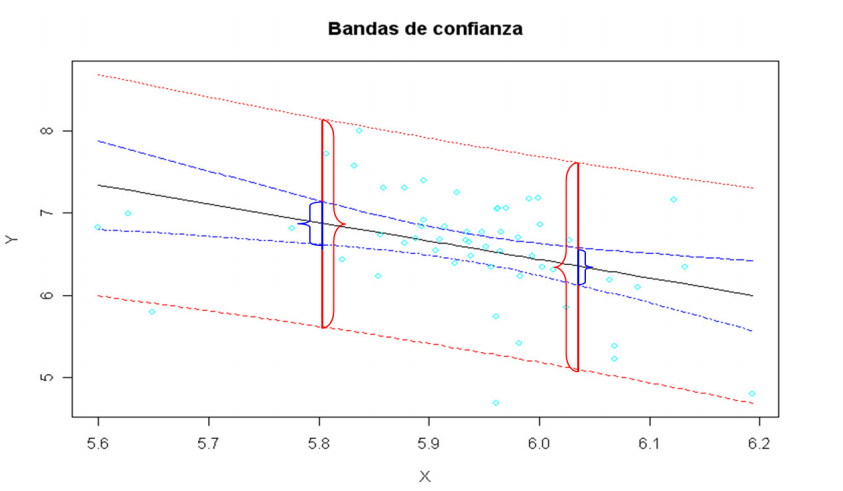
\includegraphics[scale=.7]{imagenes/tema3_4-3.png} 
\end{center}

Notemos que el aumento observado de amplitud de los intervalos de confianza al alejarnos de la media de la variable independiente es esperable, ya que las diferencias entre la pendiente estimada y la real producen errores crecientes al alejarse del centro de gravedad $(\bar{x},\bar{y})$.

Además, recordaremos que tanto la estimación de la media como de la predicción tienen una precisión que depende de $(x_p-\bar{x})^2$, por lo que es lógico que al separarnos de la media de $X$ vaya aumentando la imprecisión de las estimaciones.
	\section{Calibración Lineal}
En ocasiones el interés radica en disponer de información sobre el valor desconocido de $x_p$ para el cual se observa un valor $y_p$ de la variable dependiente. Este problema recibe el nombre de \textit{calibración lineal}.

Notemos que no tiene sentido el cálculo de la regresión de $X$ sobre $Y$ (ya que sus papeles no son intercambiables). Desde luego se puede obtener un valor para $x_p$ sin más que despejar de la expresión de la recta de regresión, pero este cálculo no es suficiente.

En efecto, dado un valor $x_p$ de la variable independiente, el intervalo de confianza para la predicción (bien sea para el valor concreto o para la media de la variable dependiente) contiene con probabilidad $1-\alpha$ al verdadero valor de la predicción. Si el valor $y_p$ observado está en ese intervalo, entonces es probable que haya sido generado por ese valor $x_p$.

Pero es probable que el valor $y_p$ también esté incluido en el intervalo generado por otro valor $x^\mathrm{'}_p$ (o por otros), con lo cual no podemos tener seguridad plena de cuál valor de la variable independiente es la generadora del valor observado de la dependiente. En consecuencia, no basta con despejar de la recta de regresión.

Según lo dicho, se puede obtener un intervalo de valores para $x_p$ sin más que igualar $y_p$ a los límites de los intervalos calculado para la predicción y despejar el valor $x_p$.

\begin{center}
IMAGEN
\end{center}

Dependiendo de que el valor $y_p$ sea considerado valor exacto o valor medio de la variable dependiente, habrá que usar unos intervalos u otros. Así para el caso del valor exacto de la variable se tiene
$$y_p=\overbrace{\bar{y}+\widehat{\beta}_1(x_p-\bar{x})}^{\widehat{y}_p}\pm t_{N-2,\frac{\alpha}{2}}\widehat{\sigma}\sqrt{1+\dfrac{1}{N}+\dfrac{(x_p-\bar{x})^2}{Ns^2_x}}$$
de donde
$$\left[(y_p-\bar{y})-\widehat{\beta}_1(x_p-\bar{x})\right]^2=t^2_{N-2,\frac{\alpha}{2}}\widehat{\sigma}^2\left(1+\dfrac{1}{N}+\dfrac{(x_p-\bar{x})^2}{Ns^2_x}\right)$$
y agrupando términos se obtiene la siguiente ecuación de segundo grado en $x_p-\bar{x}$
$$\left(\widehat{\beta}^2_1-\dfrac{t^2_{N-2,\frac{\alpha}{2}}\widehat{\sigma}^2}{Ns^2_x}\right)(x_p-\bar{x})^2-2\widehat{\beta}_1(y_p-\bar{y})(x_p-\bar{x})+(y_p-\bar{y})^2-t^2_{N-2,\frac{\alpha}{2}}\widehat{\sigma}^2\left(1+\dfrac{1}{N}\right)=0$$
cuya solución es
$$x_p-\bar{x}=\dfrac{\widehat{\beta}_1(y_p-\bar{y})}{\left(\widehat{\beta}^2_1-\dfrac{t^2_{N-2,\frac{\alpha}{2}}\widehat{\sigma}^2}{Ns^2_x}\right)}\pm\dfrac{t_{N-2,\frac{\alpha}{2}}\widehat{\sigma}\sqrt{\left(\widehat{\beta}^2_1-\dfrac{t^2_{N-2,\frac{\alpha}{2}}\widehat{\sigma}^2}{Ns^2_x}\right)\left(1+\dfrac{1}{N}\right)+\dfrac{(y_p-\bar{y})^2}{Ns^2_x}}}{\left(\widehat{\beta}^2_1-\dfrac{t^2_{N-2,\frac{\alpha}{2}}\widehat{\sigma}^2}{Ns^2_x}\right)}$$
de donde se obtiene el intervalo de valores para $x_p$
$$\bar{x}+\dfrac{\widehat{\beta}_1(y_p-\bar{y})}{\left(\widehat{\beta}^2_1-\dfrac{t^2_{N-2,\frac{\alpha}{2}}\widehat{\sigma}^2}{Ns^2_x}\right)}\pm\dfrac{t_{N-2,\frac{\alpha}{2}}\widehat{\sigma}\sqrt{\left(\widehat{\beta}^2_1-\dfrac{t^2_{N-2,\frac{\alpha}{2}}\widehat{\sigma}^2}{Ns^2_x}\right)\left(1+\dfrac{1}{N}\right)+\dfrac{(y_p-\bar{y})^2}{Ns^2_x}}}{\left(\widehat{\beta}^2_1-\dfrac{t^2_{N-2,\frac{\alpha}{2}}\widehat{\sigma}^2}{Ns^2_x}\right)}$$

Este procedimiento es válido para la obtención de un intervalo de valores para $x_p$ si el valor conocido es el promedio de la variable $x_p$ que notaremos $\bar{y}_p$. Para ello habrá que seguir el mismo proceso partiendo de la expresión del intervalo de confianza para la media de la variable dependiente, obteniéndose el intervalo
$$\bar{x}+\dfrac{\widehat{\beta}_1(y_p-\bar{y})}{\left(\widehat{\beta}^2_1-\dfrac{t^2_{N-2,\frac{\alpha}{2}}\widehat{\sigma}^2}{Ns^2_x}\right)}\pm\dfrac{t_{N-2,\frac{\alpha}{2}}\widehat{\sigma}\sqrt{\left(\widehat{\beta}^2_1-\dfrac{t^2_{N-2,\frac{\alpha}{2}}\widehat{\sigma}^2}{Ns^2_x}\right)\dfrac{1}{N}+\dfrac{(y_p-\bar{y})^2}{Ns^2_x}}}{\left(\widehat{\beta}^2_1-\dfrac{t^2_{N-2,\frac{\alpha}{2}}\widehat{\sigma}^2}{Ns^2_x}\right)}$$
\ \\

\textcolor{red}{EJERCICIO: Siguiendo el mismo razonamiento anterior, obtener el intervalo de valores para $x_p$ conocido el promedio para la variable $y_p$.}
	\section{Contraste sobre la Falta de Ajuste (o de Linealidad)}
Cuando se dispone de varios valores de la variable dependiente para cada valor fijado de la variable independiente es posible construir un contraste para investigar, la hipótesis de que las medias de las distribuciones condicionadas están o no sobre una recta. Es decir, la hipótesis nula en este caso es
$$\mathrm{H}_0:\mathrm{E}[y_{ij}\ |\ x_i]=\beta_0+\beta_1x_i$$

Sabemos que en esta situación, para cada valor de $x_i$, la distribución de $Y$ se sustituye por la media condicionada $\bar{y}_i$, lo cual introduce un error adicional en el modelo atendiendo a la representatividad de dicha media condicionada en esa distribución. Por lo tanto es esperable la existencia de dos fuentes de error: una debida a la falta de ajuste de la media condicionada a la recta, y otra debida a la variabilidad de cada distribución condicionada entorno a su media.
\end{document}
